\documentclass[a4paper,12pt,oneside,openright,extrafontsizes,openbib]{memoir}
%Define o tamanho da fonte para os título das seções primárias (Large)
\chapterstyle{section}
\renewcommand*{\chapnumfont}{\normalfont\Large\bfseries}
\renewcommand*{\chaptitlefont}{\normalfont\Large\bfseries}
%Algarismos arábicos nas páginas
\pagenumbering{arabic}
%Estilo de página
\pagestyle{simple}
%Define a PARTE (da classe Memoir) sem numeração de páginas.
\aliaspagestyle{part}{empty}
%Define secionamento numerado até a seção quaternária.
\settocdepth{subsubsection}
\setsecnumdepth{subsubsection}
%Config. das notas de rodapé.
\setlength{\footmarkwidth}{0em}
%Espaçamento de 1pt entre os parágrafos.
\setlength{\parskip}{1\baselineskip}
%Define a indentação padrão do parágrafos.
\setlength{\parindent}{1.25cm}
%Define o espaçamento entre linhas (exceto para citações longas).
\OnehalfSpacing
%========================================================
%PACOTES ESPECÍFICOS POR ÁREA DE ESTUDO/PESQUISA
%INÍCIO COMPUTAÇÃO
%Caixas de texto para inserção de códigos. Suporta diferentes linguagens.
\usepackage{codebox}
%Replicar comandos e saídas de um shell.
\usepackage{shdoc}
\shautoformat{true}
%Destacar sintaxe de código em caixa de texto simples.
\usepackage{pygmentex}
%FIM COMPUTAÇÃO
%========================================================
%Geometria do tipo de papel (A4).
\usepackage[a4paper,%
		left=3cm,%
		right=2cm,% 
		top=3cm,% 
		bottom=2cm]{geometry}
%Medir margens do pacote Geometry.
\usepackage{calc}
%Fonte 10pt para legendas de figuras e tabelas
\usepackage[font=footnotesize]{caption}
%Gerar Lorem Ipsum.
\usepackage{lipsum}
%Idiomas (o último é o principal do documento).
\usepackage[spanish,english,brazil]{babel}
%Inserir acentos .
\usepackage[utf8]{inputenc}
%Tipo de fonte usada na compilação para incluir caracteres com acentos (Ö, é, à).
\usepackage[T1]{fontenc}
%Microtipografia conforme a língua utilizada.
\usepackage[babel=true]{microtype}
%Controle e personalização de listas
\usepackage{enumitem}
\setlist{nosep}
%Hiperlinks internos e externos.
%Esconder caixa vermelha das hiperligações no documento.
%Ativar links clicáveis no pdf, com cor azul.
\usepackage[breaklinks,%
		hidelinks,%
		colorlinks=true,%
		allcolors=blue]{hyperref}
%Digitar URL completas e clicáveis. 
%Caso queira links com a cor igual ao texto (preto), mudar acima para 'colorlinks=false'.
\usepackage{xurl}
%Para escrever códigos ou trechos de códigos. Ver ambiente CODEX.
\usepackage{verbatim}
%Para escrever versos. Funciona como o verbatim.
\usepackage{alltt}
%inserir imagens.
\usepackage{graphicx}
%Inserir páginas PDF.
\usepackage{pdfpages}
%Criar multicolunas sem o ambiente "tabular".
\usepackage{multicol}
%Caixas de alerta. Útil para livros didáticos ou destaque de algum trecho importante.
\usepackage{alertmessage}
%Cores.
\usepackage{xcolor}
%Diagramas.
\usepackage{smartdiagram}
%Tabelas mais fáceis.
\usepackage{tabularx}
%Mais controle e personalização em tabelas.
\usepackage{booktabs}
%Mudar espaçamento entre linhas.
\usepackage{setspace}
%Indentação de todos os primeiros parágrafos.
\usepackage{indentfirst}
%Digitar aspas com \qq e \q.
\usepackage{textcmds}
%Fonte padrão do documento.
\usepackage{times}
%Facilidades para manipualar formatação de FONTES (riscado, espaçamento entre carcateres...).
\usepackage{soul}
%Destaca a primeira letra do parágrafo. Fonte maior e em caixa de texto.
\usepackage{lettrine}
%Símbolos fonéticos.
\usepackage{tipa}
%CAIXAS DE TEXTO
%Caixas de texto "quebráveis entre páginas".
\usepackage{mdframed}
\usepackage{framed}
%TCOLORBOXES
\usepackage{tcolorbox}
\tcbuselibrary{most,listingsutf8}

%Referências e Citações
\usepackage[alf,
            abnt-emphasize=bf,%
            abnt-etal-list=3,%
            abnt-etal-text=emph,%
            abnt-missing-year=sd,%
            abnt-repeated-author-omit=yes,%
            abnt-repeated-title-omit=yes,%
            abnt-thesis-year=final,%
            abnt-doi=link,%
            ]{abntex2cite}

%AMBIENTES PERSONALIZADOS
%Verbatim modificaddo para incluir códigos em listas.
%\newenvironment{mverbt}
%{\verbatim}%
%{\endverbatim}

%Para citações longas.
\newenvironment{citel}
{\SingleSpacing\small\list{}{\rightmargin=0cm \leftmargin=4cm}%
	\item\relax}%
{\endlist}

%Texto da folha de rosto (tipo de trabalho).
\newenvironment{textofolharosto}
{\SingleSpacing\small\list{}{\rightmargin=0cm \leftmargin=7cm}%
	\item\relax}%
{\endlist}

%Ambiente de caixa: CODEX.
\newtcblisting[auto counter,number within=chapter]{codex}[2][]{%
				arc=0mm,
				listing only,
				colback=black!5!white,
				colframe=black!85!white,
				fonttitle=\bfseries,
				title=Exemplo \thetcbcounter: #1 #2,
				listing options={style=tcblatex,%
								numbersep=1mm,%
								numbers=left,%
								numberstyle=\tiny\color{black}}
}
%Ambiente de caixa: OBSERVAÇÃO
\newtcolorbox{observ}[1][]{%
					arc=0mm,
					listing only,
					colback=black!5!white,
					colframe=red,
					fonttitle=\bfseries,
					title=Observação: #1,
}

%TCOLORBOX com molduras coloridas.
%Ambiente mvermelha
\colorlet{redbx}{red!75!black}
\newtcolorbox{mvermelha}[1]{%
	title={#1},
	empty,
	attach boxed title to top left,
	boxed title style={empty,size=minimal,
		toprule=2pt,top=4pt,
		overlay={\draw[redbx,line width=2pt]
			([yshift=-1pt]frame.north west)--([yshift=-1pt]frame.north east);}},
	coltitle=redbx,
	fonttitle=\Large\bfseries,
	before=\par\medskip\noindent,parbox=false,boxsep=0pt,left=0pt,right=3mm,top=4pt,
	breakable,pad at break*=0mm,vfill before first,
	overlay unbroken={\draw[redbx,line width=1pt]
		([yshift=-1pt]title.north east)--([xshift=-0.5pt,yshift=-1pt]title.north-|frame.east)
		--([xshift=-0.5pt]frame.south east)--(frame.south west); },
	overlay first={\draw[redbx,line width=1pt]
		([yshift=-1pt]title.north east)--([xshift=-0.5pt,yshift=-1pt]title.north-|frame.east)
		--([xshift=-0.5pt]frame.south east); },
	overlay middle={\draw[redbx,line width=1pt] ([xshift=-0.5pt]frame.north east)
		--([xshift=-0.5pt]frame.south east); },
	overlay last={\draw[redbx,line width=1pt] ([xshift=-0.5pt]frame.north east)
		--([xshift=-0.5pt]frame.south east)--(frame.south west);},%
}

%Ambiente mverde
\colorlet{greenbx}{green!75!black}
\newtcolorbox{mverde}[1]{%
	empty,title={#1},attach boxed title to top left,
	boxed title style={empty,size=minimal,toprule=2pt,top=4pt,
		overlay={\draw[greenbx,line width=2pt]
			([yshift=-1pt]frame.north west)--([yshift=-1pt]frame.north east);}},
	coltitle=greenbx,fonttitle=\Large\bfseries,
	before=\par\medskip\noindent,parbox=false,boxsep=0pt,left=0pt,right=3mm,top=4pt,
	breakable,pad at break*=0mm,vfill before first,
	overlay unbroken={\draw[greenbx,line width=1pt]
		([yshift=-1pt]title.north east)--([xshift=-0.5pt,yshift=-1pt]title.north-|frame.east)
		--([xshift=-0.5pt]frame.south east)--(frame.south west); },
	overlay first={\draw[greenbx,line width=1pt]
		([yshift=-1pt]title.north east)--([xshift=-0.5pt,yshift=-1pt]title.north-|frame.east)
		--([xshift=-0.5pt]frame.south east); },
	overlay middle={\draw[greenbx,line width=1pt] ([xshift=-0.5pt]frame.north east)
		--([xshift=-0.5pt]frame.south east); },
	overlay last={\draw[greenbx,line width=1pt] ([xshift=-0.5pt]frame.north east)
		--([xshift=-0.5pt]frame.south east)--(frame.south west);},%
}

%Caixas de textto com MDFRAMED
\newenvironment{bxpreta}
{\begin{mdframed}
		[skipabove=7pt,
		skipbelow=7pt,
		rightline=false,
		leftline=true,
		topline=false,
		bottomline=false,
		backgroundcolor=black!5,
		linecolor=black,
		innerleftmargin=5pt,
		innerrightmargin=5pt,
		innertopmargin=5pt,
		innerbottommargin=5pt,
		leftmargin=0cm,
		rightmargin=0cm,
		linewidth=5pt]}
	{\end{mdframed}}

\newenvironment{bxlaranja}
{\begin{mdframed}
		[skipabove=7pt,
		skipbelow=7pt,
		rightline=false,
		leftline=true,
		topline=false,
		bottomline=false,
		backgroundcolor=black!5,
		linecolor=orange,
		innerleftmargin=5pt,
		innerrightmargin=5pt,
		innertopmargin=5pt,
		innerbottommargin=5pt,
		leftmargin=0cm,
		rightmargin=0cm,
		linewidth=5pt]}
	{\end{mdframed}}

%Caixa Fundo cinza, Borda cinza
\newenvironment{bxcinza}
{\begin{mdframed}
		[skipabove=7pt,
		skipbelow=7pt,
		rightline=false,
		leftline=true,
		topline=false,
		bottomline=false,
		linecolor=gray,
		backgroundcolor=black!5,
		innerleftmargin=5pt,
		innerrightmargin=5pt,
		innertopmargin=5pt,
		leftmargin=0cm,
		rightmargin=0cm,
		linewidth=4pt,
		innerbottommargin=5pt]}
	{\end{mdframed}}

%Caixa Fundo azul, Borda azul
\newenvironment{bxazul}
{\begin{mdframed}
		[skipabove=7pt,
		skipbelow=7pt,
		rightline=false,
		leftline=true,
		topline=false,
		bottomline=false,
		linecolor=blue!40!gray,
		backgroundcolor=black!5,
		innerleftmargin=5pt,
		innerrightmargin=5pt,
		innertopmargin=5pt,
		leftmargin=0cm,
		rightmargin=0cm,
		linewidth=4pt,
		innerbottommargin=5pt]}
	{\end{mdframed}}

%Borda vermelha
\newenvironment{bxvermelha}
{\begin{mdframed}
		[skipabove=7pt,
		skipbelow=7pt,
		rightline=false,
		leftline=true,
		topline=false,
		bottomline=false,
		backgroundcolor=black!5,
		linecolor=red!40!gray,
		innerleftmargin=5pt,
		innerrightmargin=5pt,
		innertopmargin=5pt,
		innerbottommargin=5pt,
		leftmargin=0cm,
		rightmargin=0cm,
		linewidth=5pt]}
	{\end{mdframed}}

\begin{document}
%NÃO ALTERAR O TRECHO ABAIXO. SÃO AS CONFIGS. DOS PRÉ-TEXTUAIS.
    \begin{titlingpage}
	%PREENCHA OS CAMPOS ABAIXO COM AS INFORMAÇÕES DO SEU TRABALHO
%SUBSTITUA OS EXEMPLOS
\author{Leocádio Nestor Gumercindo Filho}
\title{A representação do arco-íris no Reino dos Unicórnios:\\ uma aplicação da variável CORES PRIMÁRIAS}
%Data da defesa. Apenas mês e ano.
\date{Jan. 2050}

%INFORMAÇÕES DA INSTITUIÇÃO E CURSO
\newcommand{\instituicao}{Instituto Federal de Pernambuco}
\newcommand{\campus}{Campus Garanhuns}
\newcommand{\curso}{Análise e desenvolvimento de sistemas}
\newcommand{\titulacao}{Tecnólogo}%Ou bacharel, ou licenciado.
\newcommand{\localdefesa}{Garanhuns - PE}
%Data exata da defesa para a folha de aprovação.
\newcommand{\dataexatadefesa}{01 de jan. \the\year}

%INFORMAÇÕES DO ORIENTADOR/A
\newcommand{\orientador}{Nome Completo do/a Orientador/a}
%Mude o texto da linha abaixo conforme o gênero do orientador/a.
\newcommand{\printorientador}{(Orientador/a)}
%Substitua "Titulação do orientador" por Esp., Me., Ma., Dr. ou Drª
\newcommand{\titorientador}{Dr.}
%Altere a linha abaixo caso seu orientador não seja do IFPE Garanhuns
\newcommand{\localorientador}{Instituto Federal de Pernambuco Campus Garanhuns}

%INFORMAÇÕES DOS AVALIADORES
%Avaliador/a 1
\newcommand{\avaliadorum}{Nome Completo do/a Avaliador/a 1}
\newcommand{\titavaliadorum}{Drª}% Esp., Me., Ma., Dr. ou Drª
\newcommand{\localavalum}{Universidade Floresta Mágica}% UFRPE, UFPE, UFMG etc por extenso
%Avaliador/a 2
\newcommand{\avaliadordois}{Nome Completo do/a Avaliador/a 1}
\newcommand{\titavaliadordois}{Me.}% Esp., Me., Ma., Dr. ou Drª
\newcommand{\localavaldois}{Instituto Bosque das Flores}% UFRPE, UFPE, UFMG etc por extenso

%FORMATAÇÃO DO ELEMENTOS PRÉ-TEXTUAIS - NÃO ALTERAR
%Capa
\begin{center}
%CAPA
%CASO NÃO DESEJE O LOGO DA INSTITUIÇÃO, EXCLUIR LINHA ABAIXO.

\includegraphics[scale=.10]{./img/logo-ifpe.png}\\
\textbf{\textsc{\instituicao}}\\
%Caso sua instituição não tenha CAMPUS, remova o comando \campus.
\textbf{\textsc{\campus}}\\
\textbf{\textsc{\curso}}


\vspace*{5cm}
\textbf{\thetitle}\\
\textbf{\theauthor}

\vspace*{\fill}
\localdefesa\\
\thedate
\end{center}

%FOLHA DE ROSTO + TIPO DE TRABALHO
\frontmatter{
\newpage
\thispagestyle{empty}
\begin{center}
    \textbf{\theauthor}
	
    \vspace*{5cm}
    \textbf{\thetitle}
\end{center}
%Caso sua instituição não tenha CAMPUS, remova o comando \campus.
%ATENÇÃO À PREPOSIÇÃO "AO/À"
\vspace*{2cm}
    \begin{textofolharosto}
    Trabalho de conclusão de curso apresentado ao/à \instituicao\ \campus\ como requisito parcial para obtenção do título de \titulacao\ em \curso.\\
    \ \\
    \textbf{Orientador:} \orientador
    \end{textofolharosto}

\begin{center}
\vspace*{\fill}
    \localdefesa\\
    \thedate
\end{center}

%FICHA CATALOGRÁFICA.
%Após a confecção da ficha catalográfica pela biblioteca de sua instituição --
%aqui, a biblioteca do IFPE Campus Garanhuns --
%imprima o arquivo (provavelmente em .docx) para pdf e salve-o
%na pasta pretxt do projeto com o nome "fichacatalografica.pdf".
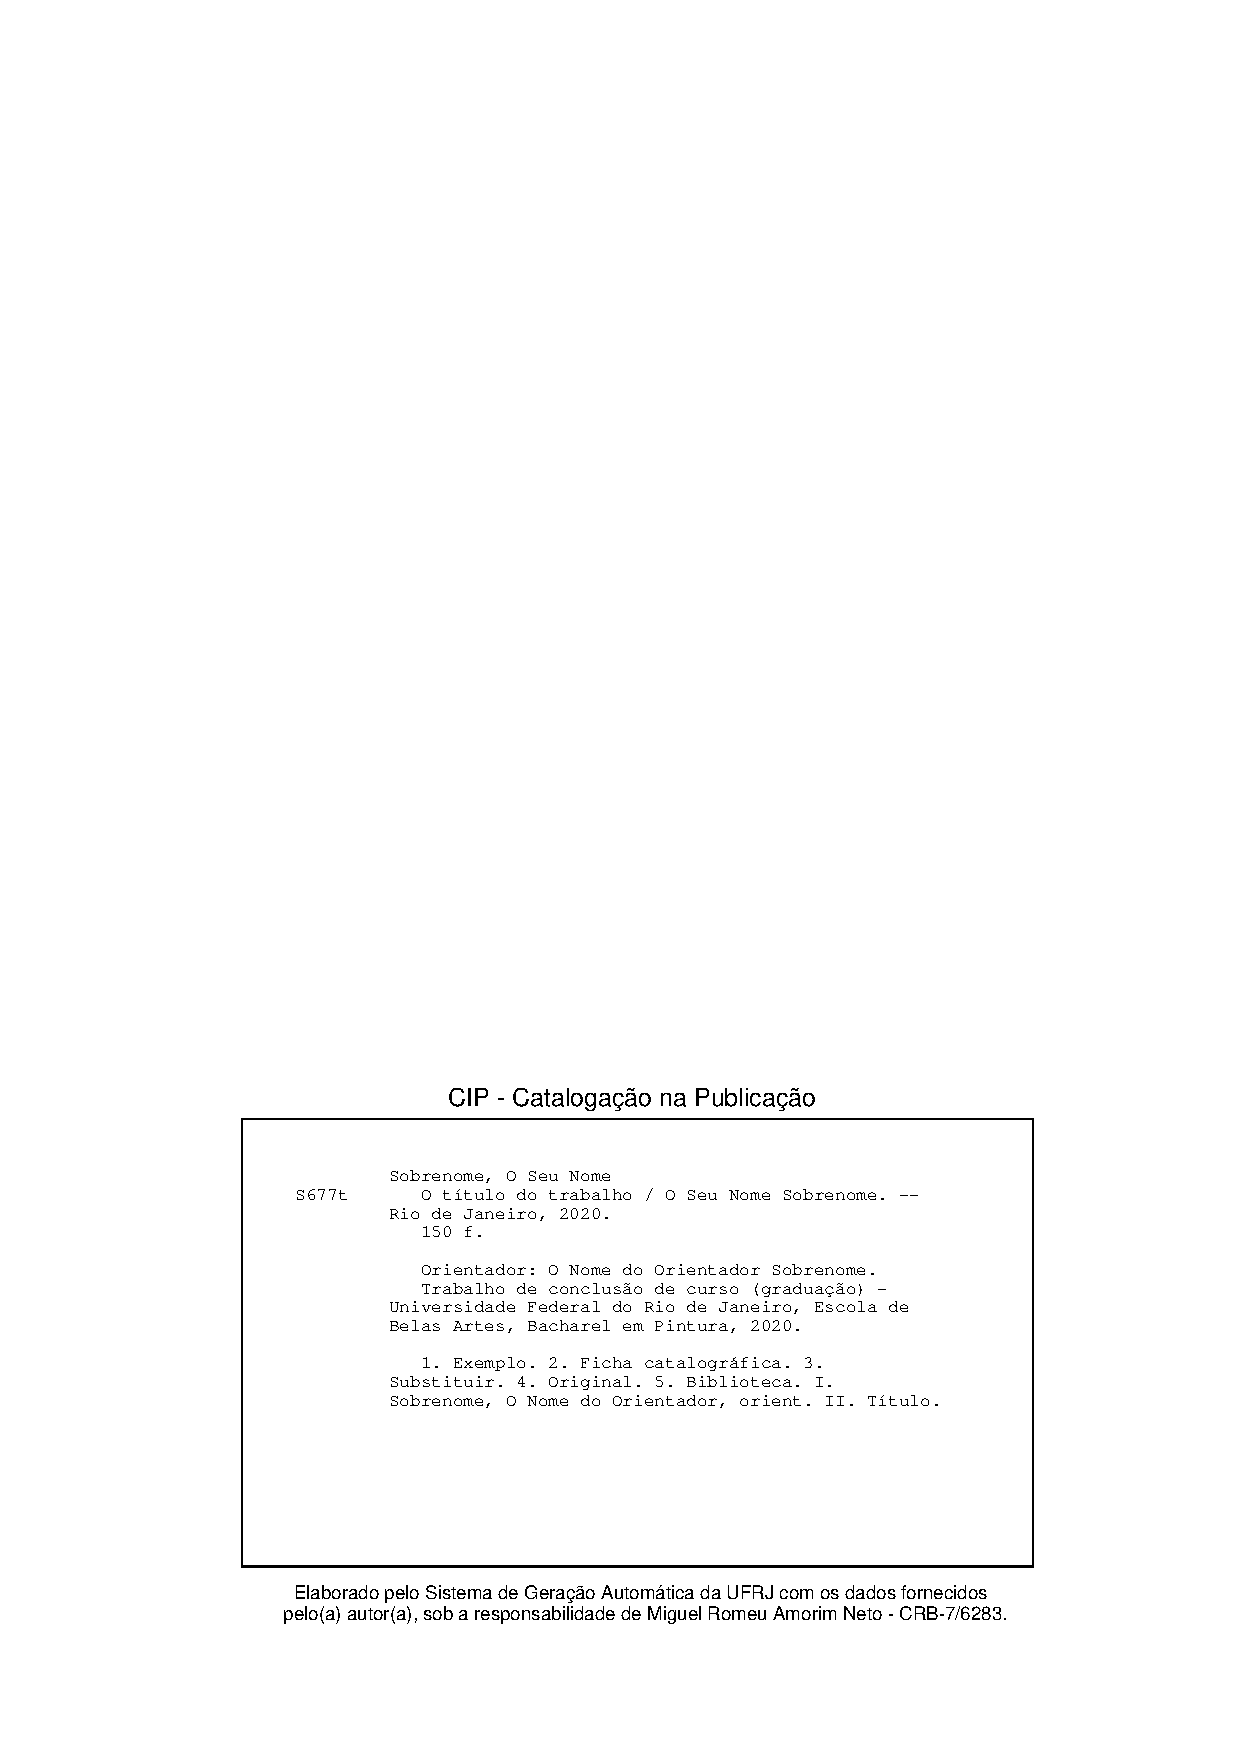
\includepdf{fichacatalografica.pdf}

%FOLHA DE APROVAÇÃO
\newpage
\thispagestyle{empty}
\begin{center}
    \textbf{\textsc{\theauthor}}
	
    \textbf{\textsc{\thetitle}}
%ATENÇÃO AO USO DA PREPOSIÇÃO (DO/DA) ANTES DO COMANDO \instituicao	
\vspace*{2cm}
    \begin{textofolharosto}
        Este Trabalho de Conclusão de Curso foi julgado adequado para obtenção do Título de \titulacao\ e aprovado em sua forma final pelo Curso de \curso\ da \instituicao\ \campus.\\
        \ \\
        \ \\
        \localdefesa\ \-- \dataexatadefesa
        \end{textofolharosto}
	
        \vspace*{2cm}
        \line(1,0){10cm}\\
        \textbf{\titorientador\ \orientador\ \printorientador}\\
        \localorientador\\
        	
        \vspace*{2cm}
        \line(1,0){10cm}\\
        \textbf{\titavaliadorum\ \avaliadorum}\\
        \localavalum\\
        	
        \vspace*{2cm}
        \line(1,0){10cm}\\
        \textbf{\titavaliadordois\ \avaliadordois}\\
        \localavaldois
    \end{center}

%EPÍGRAFE
\newpage
\thispagestyle{empty}
\vspace*{\fill}
\epigraph{\textit{Uma frase importante relacionada ao trabalho.}}{\textsc{Quem disse a frase.}}

%DEDICATÓRIA
\newpage
\thispagestyle{empty}
\vspace*{15cm}
\begin{flushright}
    \SingleSpacing\textit{Dedico este trabalho ao ilustríssimo Professor Dr. André Padilha por ter me fornecido esse modelo de trabalho em \LaTeX\ e facilitar minha jornada na escrita acadêmica.}
\end{flushright}

%AGRADECIMENTOS
\newpage
\pagestyle{empty}
\begin{center}
	\textbf{\textsc{Agradecimentos}}
\end{center}
% Digite os agradecimentos a partir da linha abaixo 
% e SEMPRE após o comando no indent, após o primeiro
% afradecimento. EXEMPLO:
Agradeço incomensuravelmente ao ilustríssimo Professor Dr. André Padilha por ter me fornecido esse modelo de trabalho em \LaTeX\ e facilitar minha jornada na escrita acadêmica.

\noindent Abaixo, o resto dos agradecimentos...

\noindent Ao papai.

\noindent À mamãe.

\noindent Ao meu papagaio José Eustáquio. 

\noindent Ao \textit{Lorem ipsum}, abaixo.

\noindent  \lipsum[10]

%RESUMO e ABSTRACT
\newpage
\pagestyle{empty}
\begin{center}
    \textbf{\textsc{Resumo}}
\end{center}
\SingleSpacing\noindent
    O resumo de um trabalho acadêmico é normatizado pela ABNT 6028:2018. Deve ser escrito em 3ª pessoa, ter entre 150 a 500 palavras e apresentar: \textit{finalidades (objetivos), metodologia, referencial teórico, resultados e conclusões}. Deve ser escrito em bloco único, com frases concisas. Para trabalhos de graduação, a prática mais comum é ter até 300 palavras.

\vspace*{0.5cm}
\noindent\textbf{Palavras-chave:} Palavra 1; Palavra 2; Palavra 3. (Até cinco, separadas por \q{ ; } (ponto e vírgula).

%ABSTRACT
\newpage
\pagestyle{empty}
\begin{center}
    \textbf{\textsc{Abstract}}
\end{center}
\SingleSpacing\noindent
    Write your abstract here. Follow the same rules as indicated previously. Avoid using any automatic translation tool as \textit{Google Translator} except if you know what you are doing.

\vspace*{0.5cm}
\noindent\textbf{Keywords:} Word 1; Word 2; Word 3.
}
\newpage
\tableofcontents*
\thispagestyle{empty}
\newpage\listoffigures*
\thispagestyle{empty}
\newpage\listoftables*
\thispagestyle{empty}
    \end{titlingpage}
%INÍCIO DOS ELEMENTOS TEXTUAIS (CAPS./SEÇÕES)
\mainmatter{
\chapter*{Apresentação}\label{ch:apres}
\addcontentsline{toc}{chapter}{Apresentação}
Este modelo de documento foi elaborado para atender às necessidades dos estudantes dos cursos de graduação do IFPE Campus Garanhuns.
Embora a biblioteca do IFPE forneça um modelo, considero sua utilização improdutiva para trabalhos acadêmicos de nível superior (graduação e pós-graduação). Não somente os aspectos diretamente relacionados à formatação, mas também em relação à estrutura do documento no tocante às seções, subseções, inserções de imagens ou tabelas com respectivas legendas e referências cruzadas são mais fáceis uma vez que se compreende o funcionamento do \LaTeX.

Também considero mais fácil o gerenciamento de referências bibliográficas e suas respectivas citações ao longo do texto, algo que no Word ou LibreOffice, por exemplo, deve ser feito com um programa externo (Zotero ou Mendeley) e seus respectivos \textit{plugins} para esses editores de texto.

Esse modelo obedece às normas ABNT eestá disponível gratuitamente no GitHub. Para aqueles que desejam realizar alguma modificação ou melhoria no modelo, sugiro que realize as mudanças diretamente no arquivo \textbf{definicoes.tex} a fim de manter a estrutura e organização do projeto. Veja o README.md no Github para explicações adicionais ou a seção 1 desse documento.

As seções desse documento contemplam os ambientes e/ou comandos mais relevantes nesse modelo, sempre seguidos de um exemplo de código e seu resultado.

%Nome do seu capítulo/seção 1. Use a ref. cruzada como em \label
\chapter{Estrutura do projeto}

Existem seis arquivos principais do projeto e uma pasta. São eles:

\begin{enumerate}
	\item \verb|definicoes.tex|
	\item \verb|pretextuais.tex|
	\item \verb|textuais.tex|
	\item \verb|postextuais.tex|
	\item \verb|referencias.bib|
	\item \verb|fichacatalografica.pdf|
	\item \verb|img|
\end{enumerate}

O arquivo \verb|definicoes.tex| contém todos os pacotes e configurações adicionais de ambientes do projeto. Essas configurações obedecem à norma ABNT NBR 14724:2011. Caso algum pacote ou configuração específica necessite inclusão, sugiro realizar nesse arquivo.

O arquivo \verb|pretextuais.tex| contém todos os elementos pré-textuais obrigatórios e opcionais conforme a norma referida acima, tais como:

\begin{itemize}
	\item Capa
	\item Folha de rosto
	\item Ficha catalográfica (ver explicação abaixo)
	\item Folha de aprovação
	\item Epígrafe
	\item Dedicatória
	\item Agradecimentos
	\item Resumo e Abstract
\end{itemize}. 

É preciso lê-lo com cuidado a fim de preencher os campos (nome do trabalho, estudante, orientador, etc) de forma adequada. No caso de não se desejar incluir os elementos opcionais (epígrafe, agradecimento, etc), basta comentar (por um sinal de \%) antes das respectivas linhas. Todos os elementos opcionais e obrigatórios estão identificados nesse arquivo.

O arquivo \verb|textuais.tex| é o arquivo em que o trabalho deve ser digitado. Deve conter todas as seções do trabalho (apresentação, seção 1, seção 2, considerações finais e referências\footnote{Ver explicação mais adiante.}).

O arquivo \verb|postextuais.tex| contém somente os elementos pós-textuais opcionais \textbf{Anexos} e \textbf{Apêndices}. As referências não estão incluídas nesse arquivo. Caso não se utilizem anexos ou apêndices, deve-se comentar a linha \verb|%ANEXOS
\thispagestyle{empty}
\part*{Anexos} % Se quiser uma página indicativa de ANEXOS antes dos anexos.
\addcontentsline{toc}{part}{Anexos}
%Conforme a norma, os anexos devem se organizar em ordem alfabética: A, B, C, D...
\chapter*{Anexo A -- Um anexo}
\addcontentsline{toc}{chapter}{Anexo A -- Um anexo}


%APÊNDICES
\thispagestyle{empty}
\part*{Apêndices} % se quiser uma página indicativa de APÊNDICES antes dos apêndices
\addcontentsline{toc}{part}{Apêndices}
%Conforme a norma, os apêndices devem se organizar em ordem alfabética: A, B, C, D...
\chapter*{Apêndice A -- lettrine}
\addcontentsline{toc}{chapter}{Apêndice A -- lettrine}

\noindent\textsc{O que faz?}

Desenha uma caixa de texto ao redor da primeira letra da primeira palavra do parágrafo. É um recurso de estilo, apenas.

\lettrine[findent=2pt]{\fbox{\textbf{V}}}{eja essa frase de abertura...} \lipsum[1]

\chapter*{Apêndice B -- verbatim}
\addcontentsline{toc}{chapter}{Apêndice A -- verbatim}

\noindent\textsc{O que faz?}

Digita qualquer coisa fora da formatação do texto, utilizando fonte monoespaçada e conforme os espaçamentos desejados. Útil para pequenos trechos de código.

\begin{codex}{Códigos verbatim}
\verb|comando 1|
    \verb*|comando 2]
        \begin{verbatim}
            qualquer outro texto
        \end{verbatim}
\begin{mverbt}
ambiente personalizado
\item um item de lista
\end{mverbt}
\end{codex}
\begin{multicols}{2}
\setlength{\columnseprule}{0.2pt}
O comando da linha 1, gera o seguinte: \verb|comando 1|.

O comando da linha 2, gera o seguinte: \verb*|comando 2].

Os comandos das linhas 3, 4 e 5 geram o seguinte:
\begin{verbatim}
   qualquer outro texto
\end{verbatim}

Os comandos das linhas 6, 7, 8 e 9 geram o seguinte:
        \begin{mverbt}
        ambiente personalizado
        \item um item de lista
        \end{mverbt}
\end{multicols}
\textbf{Observação:} Notar o alinhamento dos dois últimos ambientes. A tabulação na digitação -- \textit{em verbatim} -- importa para o \LaTeX.


\chapter*{Apêndice C -- pdfpages}
\addcontentsline{toc}{chapter}{Apêndice C -- pdfpages}

\noindent\textsc{O que faz?}

Insere uma ou várias páginas .pdf no arquivo gerado pelo \LaTeX. A numeração é feita de modo automático.

Veja a numeração desta página, note a figura inserida do Tex the Lion e a numeração do \textbf{Apêndice D}. 

Observar o código:
\ \\
\begin{codex}{Inserção de página pdf - Tex the Lion}
    
\includepdf[noautoscale=false]{img/tex-lion.pdf}
\end{codex}


\includepdf[noautoscale=false]{img/tex-lion.pdf}

\chapter*{Apêndice D -- multicol}
\addcontentsline{toc}{chapter}{Apêndice D -- multicol}

\noindent\textsc{O que faz?}

Divide o texto em -- \textit{no máximo} -- 10 colunas. No \textbf{Apêndice C}, tem-se alguns exemplos com o ambiente verbatim.

Observar:

\begin{codex}{Multicolunas com valor 3 e Lorem Ipsum}
    \begin{multicols}{3}
        \lipsum[2]
    \end{multicols}
\end{codex}

\begin{multicols}{3}
        \lipsum[2]
    \end{multicols}

\begin{codex}{Multicolunas com valor 5 e Lorem Ipsum}
    \begin{multicols}{5}
        \lipsum[2]
    \end{multicols}
\end{codex}

\begin{multicols}{5}
        \lipsum[2]
   \end{multicols}

Também é possível incluir uma linha separadora entre as colunas. Ver a seguir.

\begin{codex}{Multicolunas com valor 3 e Lorem Ipsum + Linha}
    \begin{multicols}{3}
    \setlength{\columnseprule}{0.2pt}
    \lipsum[2]
    \end{multicols}
\end{codex}

 \begin{multicols}{3}
    \setlength{\columnseprule}{0.2pt}
    \lipsum[2]
 \end{multicols}

\chapter*{Apêndice E -- smartdiagram}
\addcontentsline{toc}{chapter}{Apêndice E -- smartdiagram}

\noindent\textsc{O que faz?}

Cria diagramas coloridos, em escala de cinza, branco e preto, em formatos diversos a partir de uma lista de itens simples.

\begin{codex}{circular diagram}
\begin{center}
\smartdiagram[circular diagram]{\LaTeX,Digitar,Compilar,Produzir PDF}
\end{center}	
\end{codex}

\begin{center}
	\smartdiagram[circular diagram]{\LaTeX,Digitar,Compilar,Produzir PDF}
\end{center}

\chapter*{Apêndice F -- textcmds}
\addcontentsline{toc}{chapter}{Apêndice F -- textcmds}

\noindent\textsc{O que faz?}
Permite incluir aspas duplas e simples, e outros símbolos tipográficos, com menos esforço na digitação.

Por padrão, o \LaTeX\ produz aspas das seguintes formas:
\begin{enumerate}
	\item SHIFT + acento grave 2x + SHIFT + acento grave 2x + palavra ou expressão entre aspas + aspas simples 2x.
            \begin{itemize}
                \item 'um texto qualquer' entre aspas simples
            \end{itemize}
	\item SHIFT + sinal de acento grave + palavra ou expressão + aspas simples.
            \begin{itemize}
                \item "um texto qualquer" entre aspas duplas
            \end{itemize}
\end{enumerate}

No primeiro exemplo, o 1º sinal das aspas simples não está correto, pois deveria estar voltado para direita.

No segundo exemplo, quando compilado fora do Overleaf, não acrescenta o espaço entre as últimas aspas duplas e a próxima palavra.

Para resolver isso e utilizar \textit{on-line} e \textit{offline} ambas as aspas, use os comandos:

\begin{codex}{Aspas com o pacote textcmds}
Estas são \qq{aspas duplas}.
Estas são \q{aspas simples}.
Estas são \qq{aspas duplas com \q{aspas simples} ao mesmo tempo}
\end{codex}
 Produzirão, respectivamente: Estas são \qq{aspas duplas}; Estas são \q{aspas simples} e Estas são \qq{aspas duplas com \q{aspas simples} ao mesmo tempo}.


\chapter*{Apêndice G -- xurl}
\addcontentsline{toc}{chapter}{Apêndice G -- xurl}

\noindent\textsc{O que faz?}
Permite a quebra de \textit{urls} mesmo quando existem caracteres como \&, \_, \#.

Observe que  caixa de texto, por ser -- também -- um ambiente verbatim, não \qq{quebrará} a url, porém quando digitado em ambiente não verbatim, o endereço é ajustado automaticamente conforme as margens.

\begin{codex}{Exemplo de url longa}
  \url{https://tex.stackexchange.com/questions/341205/what-is-the-difference-between-tabular-tabular-and-tabularx-environments}
\end{codex}
\ \\
Endereço URL ajustado a seguir:

\url{https://tex.stackexchange.com/questions/341205/what-is-the-difference-between-tabular-tabular-and-tabularx-environments}

\chapter*{Apêndice H -- tabularx e booktabs}
\addcontentsline{toc}{chapter}{Apêndice H -- tabularx e booktabs}

\noindent\textsc{O que faz?}

Ambos permitem maior controle de personalização nas tabelas. Reproduzo somente uma simples tabela para fins de estudo do código.

\begin{codex}{Tabela com legenda e referência cruzada}
\begin{table}[h!]
    \begin{center}
	\begin{tabularx}{0.8\textwidth} { 
	| >{\centering\arraybackslash}X 
	| >{\centering\arraybackslash}X 
	| >{\centering\arraybackslash}X | }
	\hline
	item 1 & item 2 & item 3 \\
	\hline
	item 4  & item 5  & item 6  \\
	\hline
	\end{tabularx}
	\caption{Tabela de teste. Abaixo, a ref. cruzada.}
	\label{table:1}
	\end{center}
\end{table}
\end{codex}

\begin{table}[h!]
    \begin{center}
	\begin{tabularx}{0.8\textwidth} { 
	| >{\centering\arraybackslash}X 
	| >{\centering\arraybackslash}X 
	| >{\centering\arraybackslash}X | }
	\hline
	item 1 & item 2 & item 3 \\
	\hline
	item 4  & item 5  & item 6  \\
	\hline
	\end{tabularx}
	\caption{Tabela de teste. Abaixo, a ref. cruzada.}
	\label{table:1}
	\end{center}
\end{table}

E a ref. cruzada se faz com \verb|\ref{table:1}|, e fica \textit{hiperlinkado} para a Tabela \ref{table:1}.

\chapter*{Apêndice I -- graphix}
\addcontentsline{toc}{chapter}{Apêndice I -- graphix}

\noindent\textsc{O que faz?}

Insere imagens nos formatos JPG, PNG, PDF ou EPS. Demonstro somente como incluir uma imagem centralizada na página.

\begin{codex}{Código para inserção de imagens}
\begin{figure}[h!]
	\begin{center}
		
\includegraphics[scale=.30]{./img/github.png}
		\caption{Imagem GitHub}
		\label{fig:github}
	\end{center}
\end{figure}
\end{codex}

\begin{figure}[h!]
	\begin{center}
		
\includegraphics[scale=.30]{./img/github.png}
		\caption{Imagem GitHub}
		\label{fig:github}
	\end{center}
\end{figure}

Outras opções, tais como imagens lado a lado, aumento do tamanho, dentro de caixas de texto, etc, são indicadas no pacote.


\chapter*{Apêndice I -- Inserção de códigos de programação}
\addcontentsline{toc}{chapter}{Apêndice I -- Inserção de códigos de programação}

\noindent\textsc{O que faz?}

Insere códigos de programação com opções diferentes conforme o pacote utilizado. 

Neste modelo criei um ambiente chamado \verb|codex| que é o utilizado para todos os exemplos. Sua características são:

\begin{enumerate}
    \item caixa de texto com moldura do título preta com letras brancas
    \item texto inicial do título: \textbf{Exemplo} + \textbf{numeração da seção onde se inseriu o ambiente}
    \item fundo da caixa de texto na cor cinza
    \item numeração de linhas automáticas para análise/estudo/demonstração do código
    \item ambiente verbatim na caixa de texto
\end{enumerate} 

O ambiente \verb|codex| será o primeiro a ser exemplificado.

\textsc{Ambiente codex:} o que está dentro da primeira caixa (3.11) produzirá a segunda caixa (3.12)\footnote{Observe o espaço \textsc{intencional} entre as palavras.}.

\begin{codex}{Exemplo do exemplo}
\begin{codex}{Título de exemplo do ambiente (obrigatório)}
    aqui irá o código
        de      exemplo
    com     objetivo    de      exemplificar
\end{codex}
\end{codex}

\begin{codex}{Título de exemplo do ambiente (obrigatório)}
    aqui irá o código
        de      exemplo
    com     objetivo    de      exemplificar
\end{codex}

\newpage
\textsc{Pacote codebox}

\begin{codex}{Exemplo de uso: CODEBOX}
    \begin{codebox}{CodeBox Title}
    #include <stdio.h>
    #include <stdlib.h>
    int main(void)
    {
    printf("Hello World!\n");
    return 0;
    }
    \end{codebox}
\end{codex}

    \begin{codebox}{CodeBox Title}
    #include <stdio.h>
    #include <stdlib.h>
    int main(void)
    {
    printf("Hello World!\n");
    return 0;
    }
    \end{codebox}

\begin{codex}{Exemplo de uso: CODEVIEWER}
\begin{codeview}{CodeViewer Title}
#include <stdio.h>
#include <stdlib.h>
int main(void)
{
printf("Hello World!\n");
return 0;
}
\end{codeview}

\end{codex}
\begin{codeview}{CodeViewer Title}
#include <stdio.h>
#include <stdlib.h>
int main(void)
{
printf("Hello World!\n");
return 0;
}
\end{codeview}

\newpage
\textsc{Pacote: shdoc} (para usuários Linux)

Há diversas maneiras de utilizar o \verb|shdoc|. Utilizei um exemplo apresentado na pág. 7 do \href{https://linorg.usp.br/CTAN/macros/latex/contrib/shdoc/shdoc.pdf}{manual}.

\begin{enumerate}
    \item digitei no shell: \verb|cat --help > cat-out.save|
    \item fiz upload da saída para esse projeto
    \begin{itemize}
        \item arq. cat-out.save
    \end{itemize}
    \item executei o comando \verb|\shread{cat --help}{cat-out.save}|
    \item (não\footnote{Antes de demonstrar o pacote pygmentex (caixa acima), o Overleaf compilou o comando sem problemas e exibiu uma imagem da saída do \textit{shell}. Compatibilidade dos pacotes? Questões do Overleaf?}) obtive a imagem abaixo
\end{enumerate}

O comando \verb|\shread{cat --help}{cat-out.save}| apresentou um erro no Overleaf. Sugiro testar \textit{offline}.

\textsc{Pacote: pygmentex}

\begin{codex}{Pygmentex - pág. 2 do manual}
    \begin{pygmented}[lang=c]
    #include <stdio.h>
    int main(void)
    {
    int a, b, c;
    printf("Enter two numbers to add: ");
    scanf("%d%d", &a, &b);
    c = a + b;
    printf("Sum of entered numbers = %d\n", c);
    return 0;
    }
    \end{pygmented}
\end{codex}

O ambiente acima apresentou um erro no Overleaf. Sugiro testar \textit{offline}


\chapter*{Apêndice J -- Ambientes \LaTeX\ personalizados}
\addcontentsline{toc}{chapter}{Apêndice J -- Ambientes \LaTeX\ personalizados}

\textsc{Ambiente \textbf{citel}}
\noindent\textsc{O que faz?}

Formata as citações longas, isto é, com mais de três linhas (de acordo com a ABNT) de modo adequado no \LaTeX. Recuo de 4cm à esquerda da margem, espaçamento simples e fonte de 10pt.

\begin{codex}{Citação com blá blá}
    \begin{citel}
    blá blá blá blá blá blá blá blá blá blá blá blá blá blá blá blá blá blá blá blá blá blá blá blá blá blá blá blá blá blá blá blá blá blá blá blá blá blá blá blá blá blá blá blá blá blá blá blá blá blá blá blá blá blá blá blá blá blá blá blá blá blá blá blá blá blá blá blá blá blá blá blá blá blá blá blá blá blá blá blá blá blá blá blá blá blá blá blá blá blá blá blá blá blá blá blá blá blá blá blá blá blá blá blá blá blá blá blá blá blá blá blá blá blá blá blá blá blá blá blá blá blá blá blá blá blá blá blá blá blá (FONTE, p. 1, 2020)
\end{citel}
\end{codex}

\begin{citel}
    blá blá blá blá blá blá blá blá blá blá blá blá blá blá blá blá blá blá blá blá blá blá blá blá blá blá blá blá blá blá blá blá blá blá blá blá blá blá blá blá blá blá blá blá blá blá blá blá blá blá blá blá blá blá blá blá blá blá blá blá blá blá blá blá blá blá blá blá blá blá blá blá blá blá blá blá blá blá blá blá blá blá blá blá blá blá blá blá blá blá blá blá blá blá blá blá blá blá blá blá blá blá blá blá blá blá blá blá blá blá blá blá blá blá blá blá blá blá blá blá blá blá blá blá blá blá blá blá blá blá (FONTE, p. 1, 2020)
\end{citel}

\newpage
\textsc{Ambiente \textbf{codex}}
\noindent\textsc{O que faz?}

Ver \textbf{Apêndice I} para explicações deste ambiente.

\textsc{Ambiente \textbf{observ}}
\noindent\textsc{O que faz?}

Produz uma caixa de texto com o título "\textbf{Observação}" no topo para inserir... \textit{observações} que se julguem importantes. A fonte utilizada para o texto dentro da caixa é a mesma do documento.

\begin{codex}{Caixa para observações}
    \begin{observ}
        Aqui o texto muito importante para observações.
    \end{observ}
\end{codex}
\ \\

\begin{observ}
        Aqui o texto muito importante para observações.
    \end{observ}


\chapter*{Apêndice K -- Caixas de texto}
\addcontentsline{toc}{chapter}{Apêndice K -- Caixas de texto}

\noindent\textsc{O que faz?}

Todos os ambientes a seguir produzem caixas de texto. Em alguns trabalhos acadêmicos o \textit{corpus} é exibido com diferentes formatações e, por isso, muitas vezes precisam ser diferenciados para facilitar a leitura. 

Os ambientes nesse modelo são\footnote{Os ambientes 1 e 2 já foram exemplificados. Ver Apêndices I e J.}:

\begin{enumerate}
    \item codex
    \item observ
    \item mverde
    \item mvermelha
    \item bxpreta
    \item bxlaranja
    \item bxcinza
    \item bxazul
    \item bxvermelha
    \item \textbf{alertmessage\footnote{Exceção aos listados acima. Trata-se de um comando, não de um ambiente.}}
\end{enumerate}

Seguindo a ordem numérica acima, seguem-se os exemplos.

\begin{codex}{Ambiente mverde}
\begin{mverde}{Título da caixa mverde}
    Note que a indicação do título é obrigatória.
\end{mverde}
\end{codex}

\begin{mverde}{Título da caixa mverde}
    Note que a indicação do título é obrigatória.
\end{mverde}

\begin{codex}{Ambiente mvermelha}
\begin{mvermelha}{Título da caixa mvermelha}
    Note que a indicação do título é obrigatória.
\end{mvermelha}
\end{codex}

\begin{mvermelha}{Título da caixa mvermelha}
    Note que a indicação do título é obrigatória.
\end{mvermelha}

\textsc{Atenção:} para as caixas/os ambientes \verb|mverde| e \verb|mvermelha| o texto do título é obrigatório.

As caixas seguintes não requerem título. Primeiro apresenta-se o código, em seguida o que é produzido/gerado para o pdf.

\begin{codex}{Ambiente bxpreta}
\begin{bxpreta}
Caixa de texto com moldura preta na lateral esquerda.    
\end{bxpreta} 
\end{codex}
.
\begin{bxpreta}
Caixa de texto com \textbf{moldura preta} na lateral esquerda.    
\end{bxpreta} 

\begin{codex}{Ambiente bxlaranja}
    \begin{bxlaranja}
        Caixa de texto com \textbf{moldura laranja} na lateral esquerda.  
    \end{bxlaranja}
 \end{codex}
.
\begin{bxlaranja}
        Caixa de texto com \textbf{moldura laranja} na lateral esquerda.  
\end{bxlaranja}


\begin{codex}{Ambiente bxcinza}
    \begin{bxcinza}
      Caixa de texto com \textbf{moldura cinza} na lateral esquerda. 
    \end{bxcinza}
\end{codex}
.
\begin{bxcinza}
      Caixa de texto com \textbf{moldura cinza} na lateral esquerda. 
\end{bxcinza}


\begin{codex}{Ambiente bxazul}
    \begin{bxazul}
      Caixa de texto com \textbf{moldura azul} na lateral esquerda. 
    \end{bxazul}
\end{codex}
.
\begin{bxazul}
      Caixa de texto com \textbf{moldura azul} na lateral esquerda. 
\end{bxazul}

\begin{codex}{Ambiente bxvermelha}
    \begin{bxvermelha}
      Caixa de texto com \textbf{moldura vermelha} na lateral esquerda. 
    \end{bxvermelha}
\end{codex}
.
\begin{bxvermelha}
   Caixa de texto com \textbf{moldura vermelha} na lateral esquerda. 
\end{bxvermelha}

Os últimos exemplos não são ambientes, mas comandos do pacote \verb|alertmessage| incluído nesse modelo de documento.

\begin{codex}{Todos os comandos para alertmessage}
    A. \alertinfo{caixa azul, com ícone "i"}
    B. \alertsuccess{caixa verde com ícone de "confere"}
    C. \alerterror{caixa vermelha com ícone de "x" ou "erro"}
    D. \alertwarning{caixa laranja com ícone de"!" ou exclamação}
\end{codex}

    A. \alertinfo{caixa azul, com ícone "i".}

    B. \alertsuccess{caixa verde com ícone de "confere".}
    
    C. \alerterror{caixa vermelha com ícone de "x" ou "erro".}
    
    D. \alertwarning{caixa laranja com íncone de"!" ou exclamação.}| ao final \underline{deste} arquivo (textuais.tex).

Observe que as \textbf{referências} são elementos pós-textuais. No entanto, o \LaTeX, especificamente o pacote \textit{Memoir}, no qual esse modelo se baseia, divide as partes do documento em \verb|\frontmatter| (está no pretextuais.tex), \verb|\maintmatter| (está no início desse arquivo) e \verb|\backmatter| (está no final deste arquivo). Como as referências, que são obrigatórias, antecedem anexos e/ou apêndices, para facilitar a organização, incluí a indicação de onde se localiza o arquivo com as referências aqui, no \verb|textuais.tex| porque, se inexistirem anexos e apêndices, basta comentar a linha respectiva (ver instrução acima) sem prejuízo às referências.

O arquivo \verb|referencias.bib| é o arquivo com todas as referências utilizadas no trabalho. Esse arquivo funciona como um banco de dados. O \LaTeX\ lê cada uma das entradas (livro, artigo, capítulo de livro, manual, etc) e faz a compilação no formato da ABNT NBR 6023:2018. Existem entradas já preenchidas que servem como modelos e, também, entradas em branco para facilitar o copia+cola. Veja mais atentamente a seção \textbf{Referências}, pois lá existem explicações mais detalhadas.

O arquivo \verb|fichacatalografica.pdf| serve apenas para a compilação, durante a escrita do trabalho, não dar erro. Esse arquivo é criado pelo/a bibliotecário/a do campus (ou instituição, caso não seja o IFPE) ao final do trabalho (após a defesa). Deve ser convertido para .pdf e nomeado como \textbf{fichacatalografica.pdf}. Em seguida, copia-se esse arquivo em .pdf para a pasta do projeto de modo a substituir o arquivo existente. Depois, compila-se normalmente e \textit{voilá}, tudo pronto para o depósito no RI.

A pasta \verb|img| é onde devem ser colocadas todas as imagens (caso as utilize) do trabalho. No momento da inclusão da imagem no arquivo, o caminho da imagem deve ser relativo, por exemplo\footnote{Ver instruções específicas na seção Imagens.}: comando-para-imagem\{./img/nome-da-imagem.png\}.Deve-se sempre  indicar a extensão da imagem: png, jpg, jpeg, etc.

Cada uma das seções inicia-se com uma pergunta: \textbf{Qual o pacote?}, cuja resposta indica o endereço URL do pacote no CTAN (Comprenhensive \TeX Archive Network), um repositório de todos os pacotes do \LaTeX, bem como a documentação de cada um. Em seguida, outra pergunta: \textbf{O que faz?}, indicando o que aquele pacote, incluído nesse modelo, faz em termos de formatação. Depois, temos uma caixa com o código e, em seguida, o resultado daquele código.
%=======================================================
\chapter{Lettrine}

\textsc{Qual o pacote?}: \textbf{lettrine} (\url{https://www.ctan.org/pkg/lettrine})

\textsc{O que faz?}: Desenha uma caixa de texto ao redor da primeira letra da primeira palavra do parágrafo. É um recurso de estilo, apenas.

\begin{codex}{Código pacote lettrine}
\lettrine[findent=2pt]{\fbox{\textbf{V}}}{eja essa frase de abertura...} \lipsum[1]
\end{codex}

\textsc{Resultado}:

\lettrine[findent=2pt]{\fbox{\textbf{V}}}{eja essa frase de abertura...} \lipsum[1]
 
%=======================================================
\chapter{Verbatim}

\textsc{Qual o pacote?}: \textbf{verbatim}\footnote{Por padrão, já incluído no \LaTeX.} (Acesso: \url{https://www.ctan.org/pkg/verbatim})

\textsc{O que faz?}: Digita qualquer coisa fora da formatação do texto, utilizando fonte monoespaçada e conforme os espaçamentos desejados. Útil para pequenos trechos de código.

\begin{codex}{Códigos ambiente verbatim}
	\verb|comando 1|
	\verb*|comando 2]|
	\begin{verbatim}
		qualquer outro texto
	\end{verbatim}
\end{codex}

\textsc{Resultado}:

\verb|comando 1|

\verb*|comando 2]|

\begin{verbatim}
	qualquer outro texto
	e outro texto qualquer
\end{verbatim}

\textbf{Importante:} O ambiente verbatim não respeitas as margens. Isto quer dizer que se tudo for digitado em uma única linha, sem quebra manual, ele irá mostrar o texto quebrado. Observe:

\begin{verbatim}
	Stricto sensu é uma expressão latina que significa, literalmente, "em sentido específico", por oposição ao "sentido amplo" de um termo. No âmbito do ensino, se refere ao nível de pós-graduação que titula o estudante como mestre ou doutor em determinado campo do conhecimento. Denota, neste caso, um grau mais elevado do que a pesquisa lato sensu.
\end{verbatim}

O código acima é:

\begin{codex}{Código verbatim sem quebra de linha}
	Stricto sensu é uma expressão latina que significa, literalmente, "em sentido específico", por oposição ao "sentido amplo" de um termo. No âmbito do ensino, se refere ao nível de pós-graduação que titula o estudante como mestre ou doutor em determinado campo do conhecimento. Denota, neste caso, um grau mais elevado do que a pesquisa lato sensu.
\end{codex}
%=======================================================
\chapter{Inserir páginas em .pdf}

\textsc{Qual o pacote?}: \textbf{pdfpages} (Acesso: \url{https://www.ctan.org/pkg/pdfpages})

\textsc{O que faz?}: Insere uma ou várias páginas .pdf no arquivo gerado pelo \LaTeX. A numeração é feita de modo automático.

Veja a numeração desta página, note a figura inserida do Tex the Lion e a numeração da página após a inserção do arquivo .pdf.
\ \\

\begin{codex}{Código inserção de página pdf. Imagen: Tex the Lion}
	
\includepdf[noautoscale=false]{img/tex-lion.pdf}
\end{codex}

\textsc{Resultado}:


\includepdf[noautoscale=false]{img/tex-lion.pdf}
%=======================================================
\chapter{Texto em várias colunas}

\textsc{Qual o pacote:} \textbf{multicol} (Acesso: \url{https://www.ctan.org/pkg/multicol})

\textsc{O que faz?}: Divide o texto em colunas (Máx. de 10 colunas.)

\begin{codex}{Código multicolunas com valor 3 e Lorem Ipsum}
	\begin{multicols}{3}
		\lipsum[2]
	\end{multicols}
\end{codex}

\textsc{Resultado}:

\begin{multicols}{3}
	\lipsum[2]
\end{multicols}

\begin{codex}{Código multicolunas com valor 5 e Lorem Ipsum}
	\begin{multicols}{5}
		\lipsum[2]
	\end{multicols}
\end{codex}

\textsc{Resultado}:

\begin{multicols}{5}
	\lipsum[2]
\end{multicols}

Também é possível incluir uma linha separadora entre as colunas. Ver a seguir.

\begin{codex}{Código multicolunas com valor 3 e Lorem Ipsum + Linha}
	\begin{multicols}{3}
		\setlength{\columnseprule}{0.2pt}
		\lipsum[2]
	\end{multicols}
\end{codex}

\textsc{Resultado}:

\begin{multicols}{3}
	\setlength{\columnseprule}{0.2pt}
	\lipsum[2]
\end{multicols}

Veja também \url{https://www.alessandroduarte.com.br/?page_id=602} para um tutorial em português.
%=======================================================
\chapter{Diagramas}

\textsc{Pacote:} \textbf{smartdiagram} (Acesso: \url{https://www.ctan.org/pkg/smartdiagram})

\textsc{O que faz?}: Cria diagramas coloridos, em escala de cinza, branco e preto, em formatos diversos a partir de uma lista de itens simples.

\begin{codex}{Código para diagrama circular}
	\begin{center}
		\smartdiagram[circular diagram]{\LaTeX,Digitar,Compilar,Produzir PDF}
	\end{center}	
\end{codex}

\textsc{Resultado}:

\begin{center}
	\smartdiagram[circular diagram]{\LaTeX,Digitar,Compilar,Produzir PDF}
\end{center}

\begin{codex}{Código para diagrama descritivo}
\smartdiagram[descriptive diagram]{
	{Set up,The set up operation consist of..},
	{Run, {After having set up the program, you must run..}},
	{Analyse, You must check what did with analytical tools like..},
	{Modify, {After the analysis, you can still modify or add..}},
}
\end{codex}

\textsc{Resultado:}

\begin{center}
	\smartdiagram[descriptive diagram]{
		{Set up,The set up operation consist of..},
		{Run, {After having set up the program, you must run..}},
		{Analyse, You must check what did with analytical tools like..},
		{Modify, {After the analysis, you can still modify or add..}},
	}
\end{center}


%=======================================================
\chapter{Aspas e outros símbolos tipográficos}

\textsc{Pacote:} \textbf{textcmds} (Acesso: \url{https://ctan.math.illinois.edu/macros/latex/contrib/amsrefs/textcmds.pdf})

\textsc{O que faz?}: Permite incluir aspas duplas e simples, e outros símbolos tipográficos, com menos esforço na digitação. Ver explicação a seguir.

Por padrão, o \LaTeX\ produz aspas das seguintes formas:

\begin{enumerate}
	\item SHIFT + acento grave 2x + SHIFT + acento grave 2x + palavra ou expressão entre aspas + aspas simples 2x.
	\begin{itemize}
		\item 'um texto qualquer' entre aspas simples
	\end{itemize}
	\item SHIFT + sinal de acento grave + palavra ou expressão + aspas simples.
	\begin{itemize}
		\item "um texto qualquer" entre aspas duplas
	\end{itemize}
\end{enumerate}

No primeiro exemplo, o 1º sinal das aspas simples não está correto, pois deveria estar voltado para direita.

No segundo exemplo, não acrescenta o espaço entre as últimas aspas duplas e a próxima palavra.

Para resolver isso e utilizar ambas as aspas corretamente, use os comandos:

\begin{codex}{Códigos para aspas com o pacote textcmds}
	Estas são \qq{aspas duplas}.
	Estas são \q{aspas simples}.
	Estas são \qq{aspas duplas com \q{aspas simples} ao mesmo tempo}
\end{codex}

\textsc{Resultado}:

Estas são \qq{aspas duplas}; Estas são \q{aspas simples} e estas são \qq{aspas duplas com \q{aspas simples} ao mesmo tempo}.

Esse pacote foi incluído porque em modo \textit{offline} o \LaTeX\ habitualmente não reconhece os espaços necessários entre as aspas.
%=======================================================
\chapter{Hiperlinks com quebra de endereço por linha}

\textsc{Qual o pacote?} \textbf{xurl} (Acesso: \url{https://www.ctan.org/pkg/xurl})

\textsc{O que faz?}: Permite a quebra de \textit{urls} mesmo quando, no endereço, existem caracteres como \&, \_, \#.

Observe que, por ser -- também -- um ambiente verbatim, não \qq{quebrará} a url, porém quando digitado em ambiente não verbatim, o endereço é ajustado automaticamente conforme as margens.

\begin{codex}{Código de exemplo de url longa}
\url{https://tex.stackexchange.com/questions/341205/what-is-the-difference-between-tabular-tabular-and-tabularx-environments}
\end{codex}
\ \\

\textsc{Resultado:}

\url{https://tex.stackexchange.com/questions/341205/what-is-the-difference-between-tabular-tabular-and-tabularx-environments}

%=======================================================
\chapter{Tabelas}

\textsc{Quais os pacotes?} \textbf{tabularx} (Acesso: \url{https://www.ctan.org/pkg/tabularx}) e \textbf{booktabs} (Acesso: \url{https://www.ctan.org/pkg/booktabs/}).

\textsc{O que fazem?}: Ambos permitem maior controle de personalização nas tabelas. 

Relevante observar que tabelas, \textit{stricto sensu}, são elementos destinados a apresentar dados \textbf{numéricos} e não apresentam linhas laterais. Temos o costume, aqui no Brasil, de incluir tais linhas, inserir outros dados que não sejam numéricos e identificar o elemento como tabela. Esse é um procedimento incorreto. 

Caso se apresentem dados não numéricos e linhas laterais, deve-se identificar esse elementos como \textsc{quadro}.

Veja a seguir um exemplo de como normalmente se faz no Brasil\footnote{Obviamente que fica a critério da pessoa que elabora o trabalho optar pela forma abaixo ou não.}.

\begin{codex}{Código para tabela com legenda e referência cruzada}
\begin{table}[h!]
	\begin{center}
	\begin{tabularx}{0.8\textwidth} { 
	| >{\centering\arraybackslash}X 
	| >{\centering\arraybackslash}X 
	| >{\centering\arraybackslash}X | }
	\hline
	item 1 & item 2 & item 3 \\
	\hline
	item 4  & item 5  & item 6  \\
	\hline
	\end{tabularx}
	\caption{Tabela de teste com linhas laterais.}
	\label{table:1}
	\end{center}
	\end{table}
\end{codex}

\textsc{Resultado:}

\begin{table}[h!]
	\begin{center}
		\begin{tabularx}{0.8\textwidth} { 
				| >{\centering\arraybackslash}X 
				| >{\centering\arraybackslash}X 
				| >{\centering\arraybackslash}X | }
			\hline
			item 1 & item 2 & item 3 \\
			\hline
			item 4  & item 5  & item 6  \\
			\hline
		\end{tabularx}
		\caption{Tabela de teste com linhas laterais.}
		\label{table:1}
	\end{center}
\end{table}

E para referenciar a tabela/quadro, usamos o comando \verb|\ref{table:1}|, como abaixo.

Ex.: \textit{Como podemos observar na tabela \ref{table:1}, blá blá...}

No entanto, a correta aplicação e formatação de uma tabela deve ser conforme o código a seguir.

\begin{codex}{Código de exemplo de tabela}
	\begin{table}[h!]
	\begin{center}
	\begin{tabular}{c|c|c|c}
	\hline
	Percentual & 15\% & 37\% & 50\% \\
	\hline
	Número & 23 & 44 & 71 \\
	\hline
	Variação & 2.78 & 4.59 & 10.96 \\
	\hline
	Total & > 3 & < 8 & >15  \\
	\hline
	\end{tabular}
	\caption{Tabela de teste sem linhas laterais. Abaixo, a ref. cruzada.}
	\label{table:2}
	\end{center}
	\end{table}
\end{codex}

\textsc{Resultado:}

\begin{table}[h!]
	\begin{center}
		\begin{tabular}{c|c|c|c}
			\hline
			Percentual & 15\% & 37\% & 50\% \\
			\hline
			Número & 23 & 44 & 71 \\
			\hline
			Variação & 2.78 & 4.59 & 10.96 \\
			\hline
			Total & > 3 & < 8 & >15  \\
			\hline
		\end{tabular}
		\caption{Tabela de teste sem linhas laterais. Abaixo, a ref. cruzada.}
		\label{table:2}
	\end{center}
\end{table}

E, como acima, referenciamos a tabela (ref. cruzada) com o comando \verb|\ref{table:2}|.

Ex.: \textit{Como podemos observar na tabela \ref{table:2}, blá blá...}

A lista de tabela, quando identificadas pelos dois comandos \verb|\caption{...}| e \verb|\label{...}| já são inseridas automaticamente na seção \textbf{Lista de tabelas}.

Tabelas em \LaTeX\ são incrivelmente \qq{complicadas} de fazer. Sugiro abaixo uma breve lista com geradores de códigos de tabela em \LaTeX\ \textit{on-line}.

\begin{enumerate}
	\item \url{https://www.tablesgenerator.com/}
	\item \url{https://www.latex-tables.com/}
	\item \url{https://clevert.com.br/latex/latextable.php}
\end{enumerate}

Por fim, ao final do arquivo \verb|pretextuais.tex|, há os seguintes códigos:

\begin{codex}{Códigos para tabelas e figuras}
	\newpage\tableofcontents*
	\thispagestyle{empty}
	\newpage\listoffigures*
	\thispagestyle{empty}
	\newpage\listoftables*
	\thispagestyle{empty}
\end{codex}

Caso não existam nem figuras nem tabelas no trabalho, basta excluir as linhas: 
\begin{verbatim} 
	\newpage\listoffigures*
	\thispagestyle{empty}
	\newpage\listoftables*
	\thispagestyle{empty} 
\end{verbatim}

%=======================================================
\chapter{Imagens}

\textsc{Qual o pacote?} \textbf{graphicx} (Acesso: \url{https://www.ctan.org/pkg/graphicx})

\textsc{O que faz?}: Insere imagens nos formatos JPG, PNG, PDF ou EPS. Demonstro somente como incluir uma imagem centralizada na página.

\begin{codex}{Código para inserção de imagens}
\begin{figure}[h!]
\begin{center}

\includegraphics[scale=.30]{./img/github.png}
\caption{Imagem GitHub}
\label{fig:github}
\end{center}
\end{figure}
\end{codex}

\textsc{Resultado:}

\begin{figure}[h!]
	\begin{center}
		
\includegraphics[scale=.30]{./img/github.png}
		\caption{Imagem GitHub}
		\label{fig:github}
	\end{center}
\end{figure}

Uma demonstração combinada com o uso do pacote \textbf{multicol} dispondo as figuras lado a lado.

\begin{codex}{Código para figuras lado a lado com multicol}
\begin{multicols}{2}

\includegraphics[scale=.15]{./img/github.png}

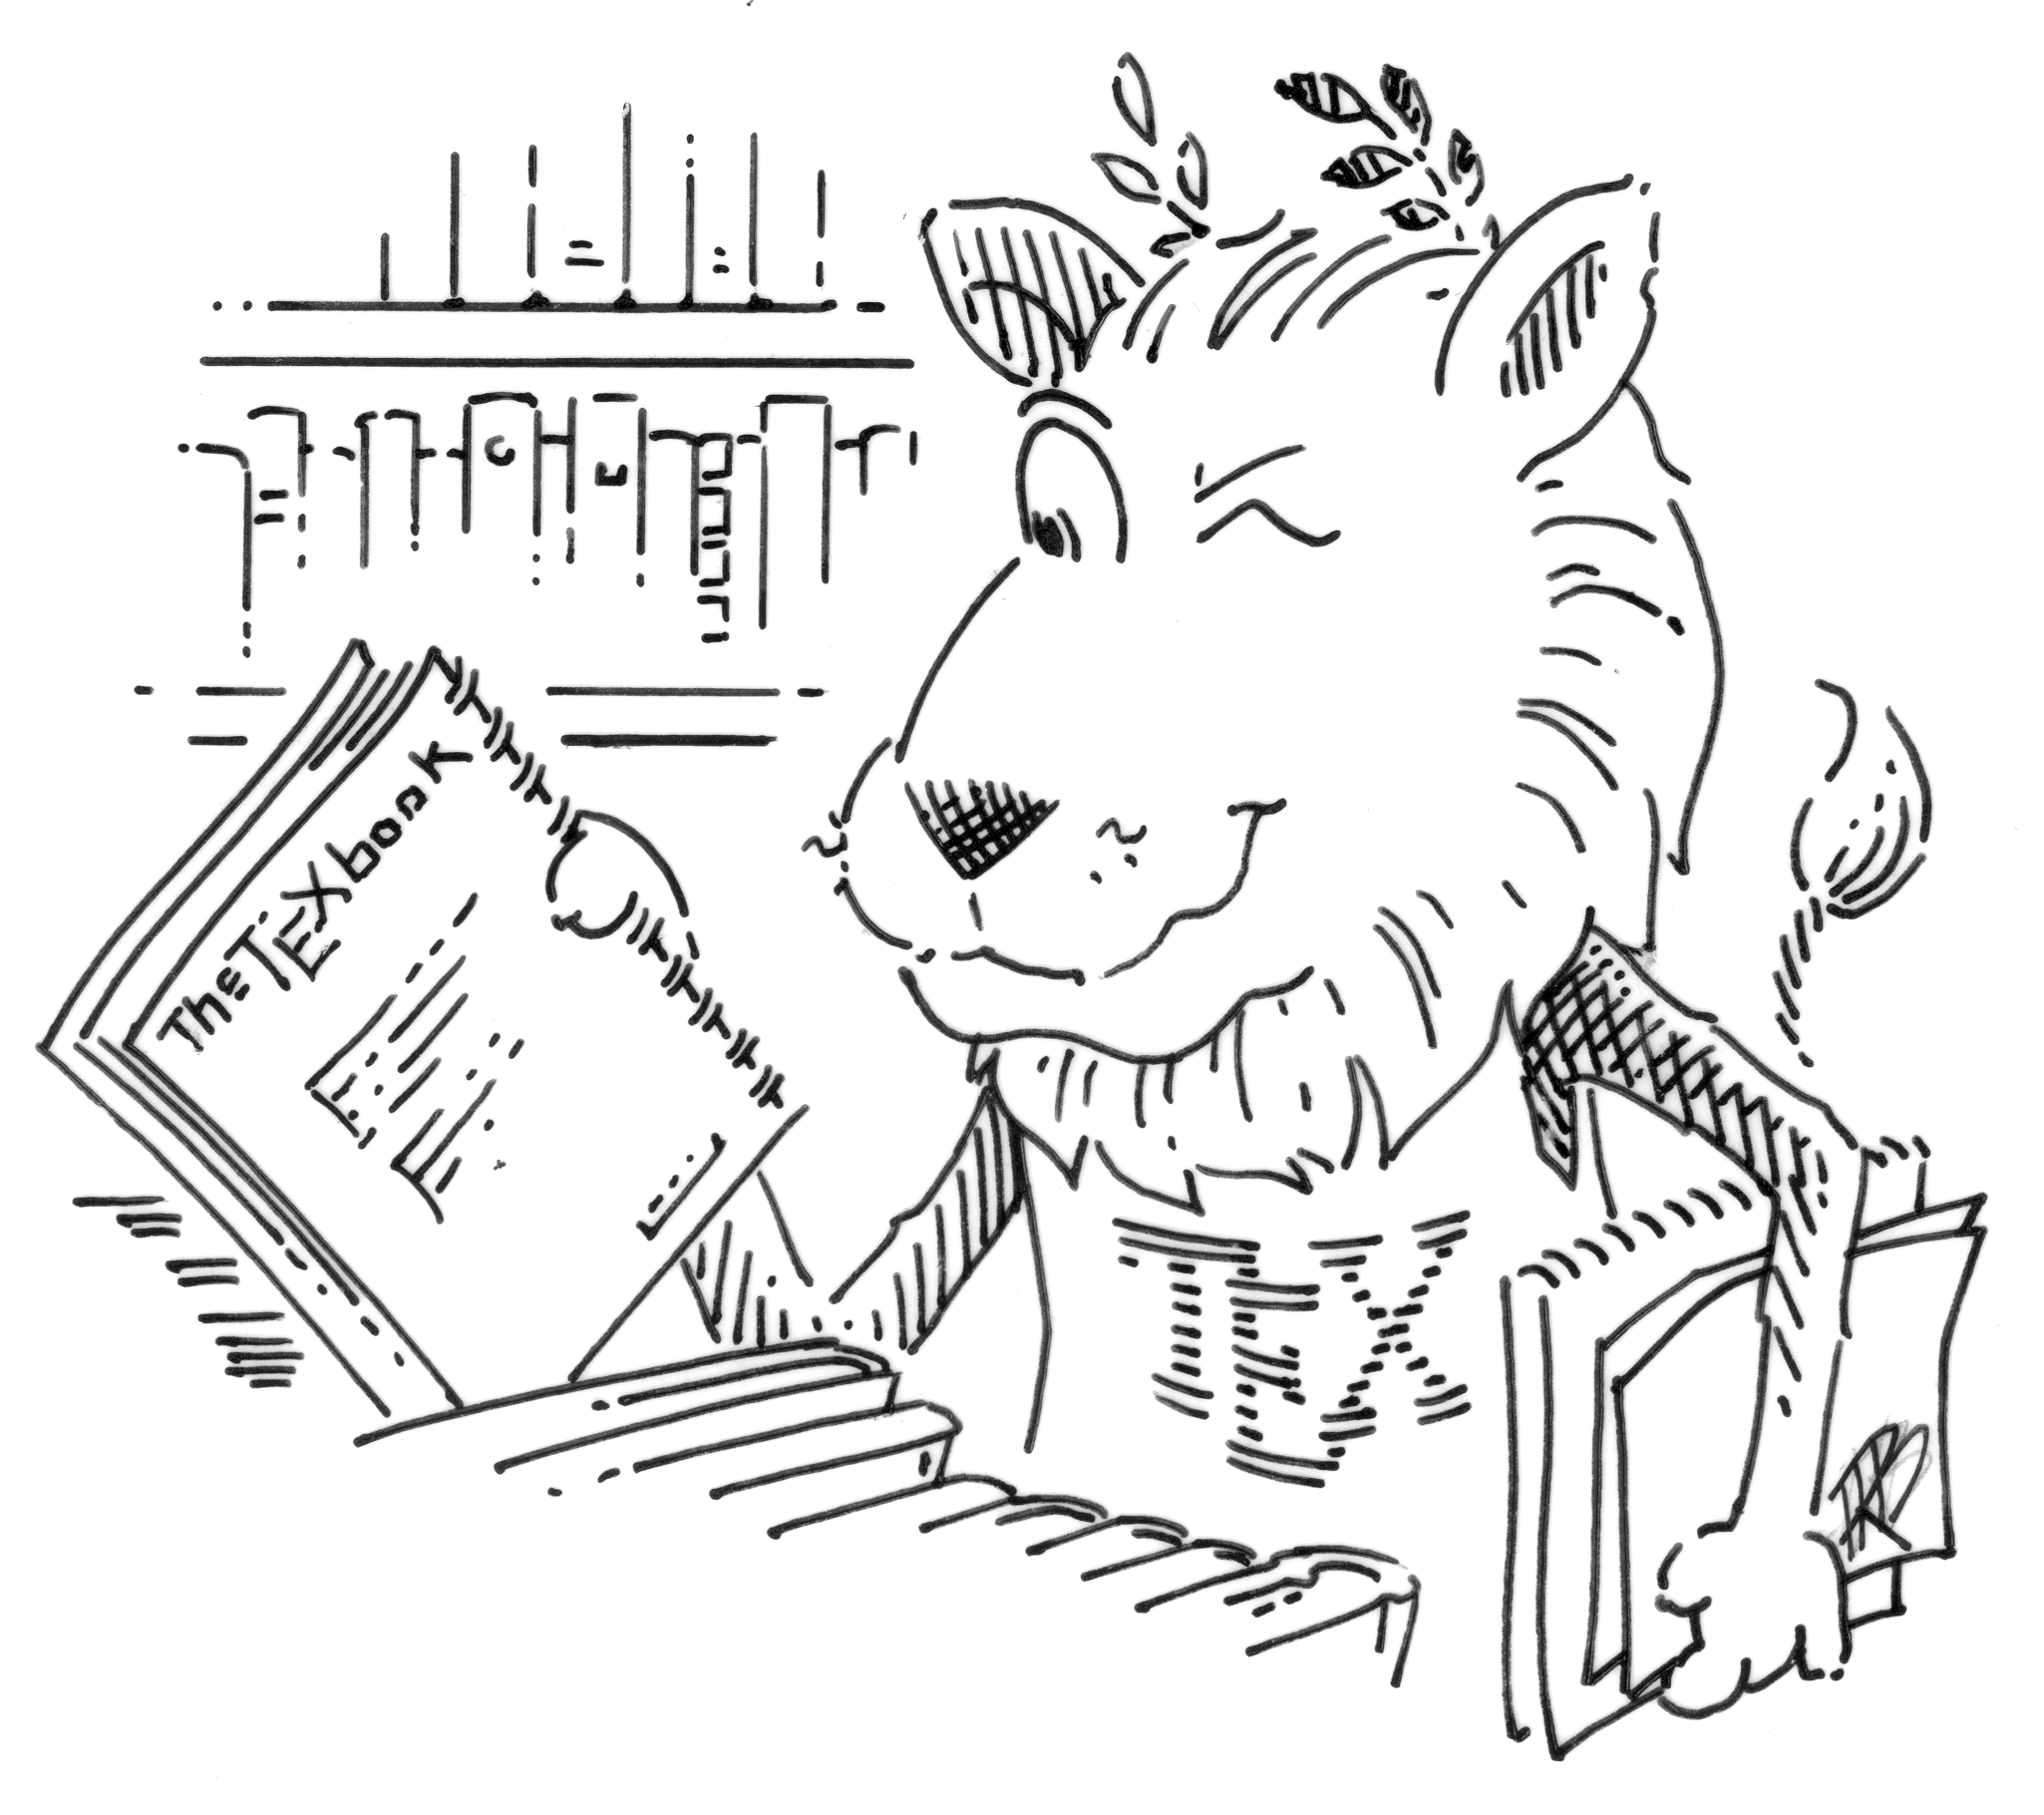
\includegraphics[scale=.040]{./img/tex-lion.png}
\end{multicols}
\end{codex}

\textsc{Resultado:}
\begin{multicols}{2}
	
\includegraphics[scale=.15]{./img/github.png}
	
	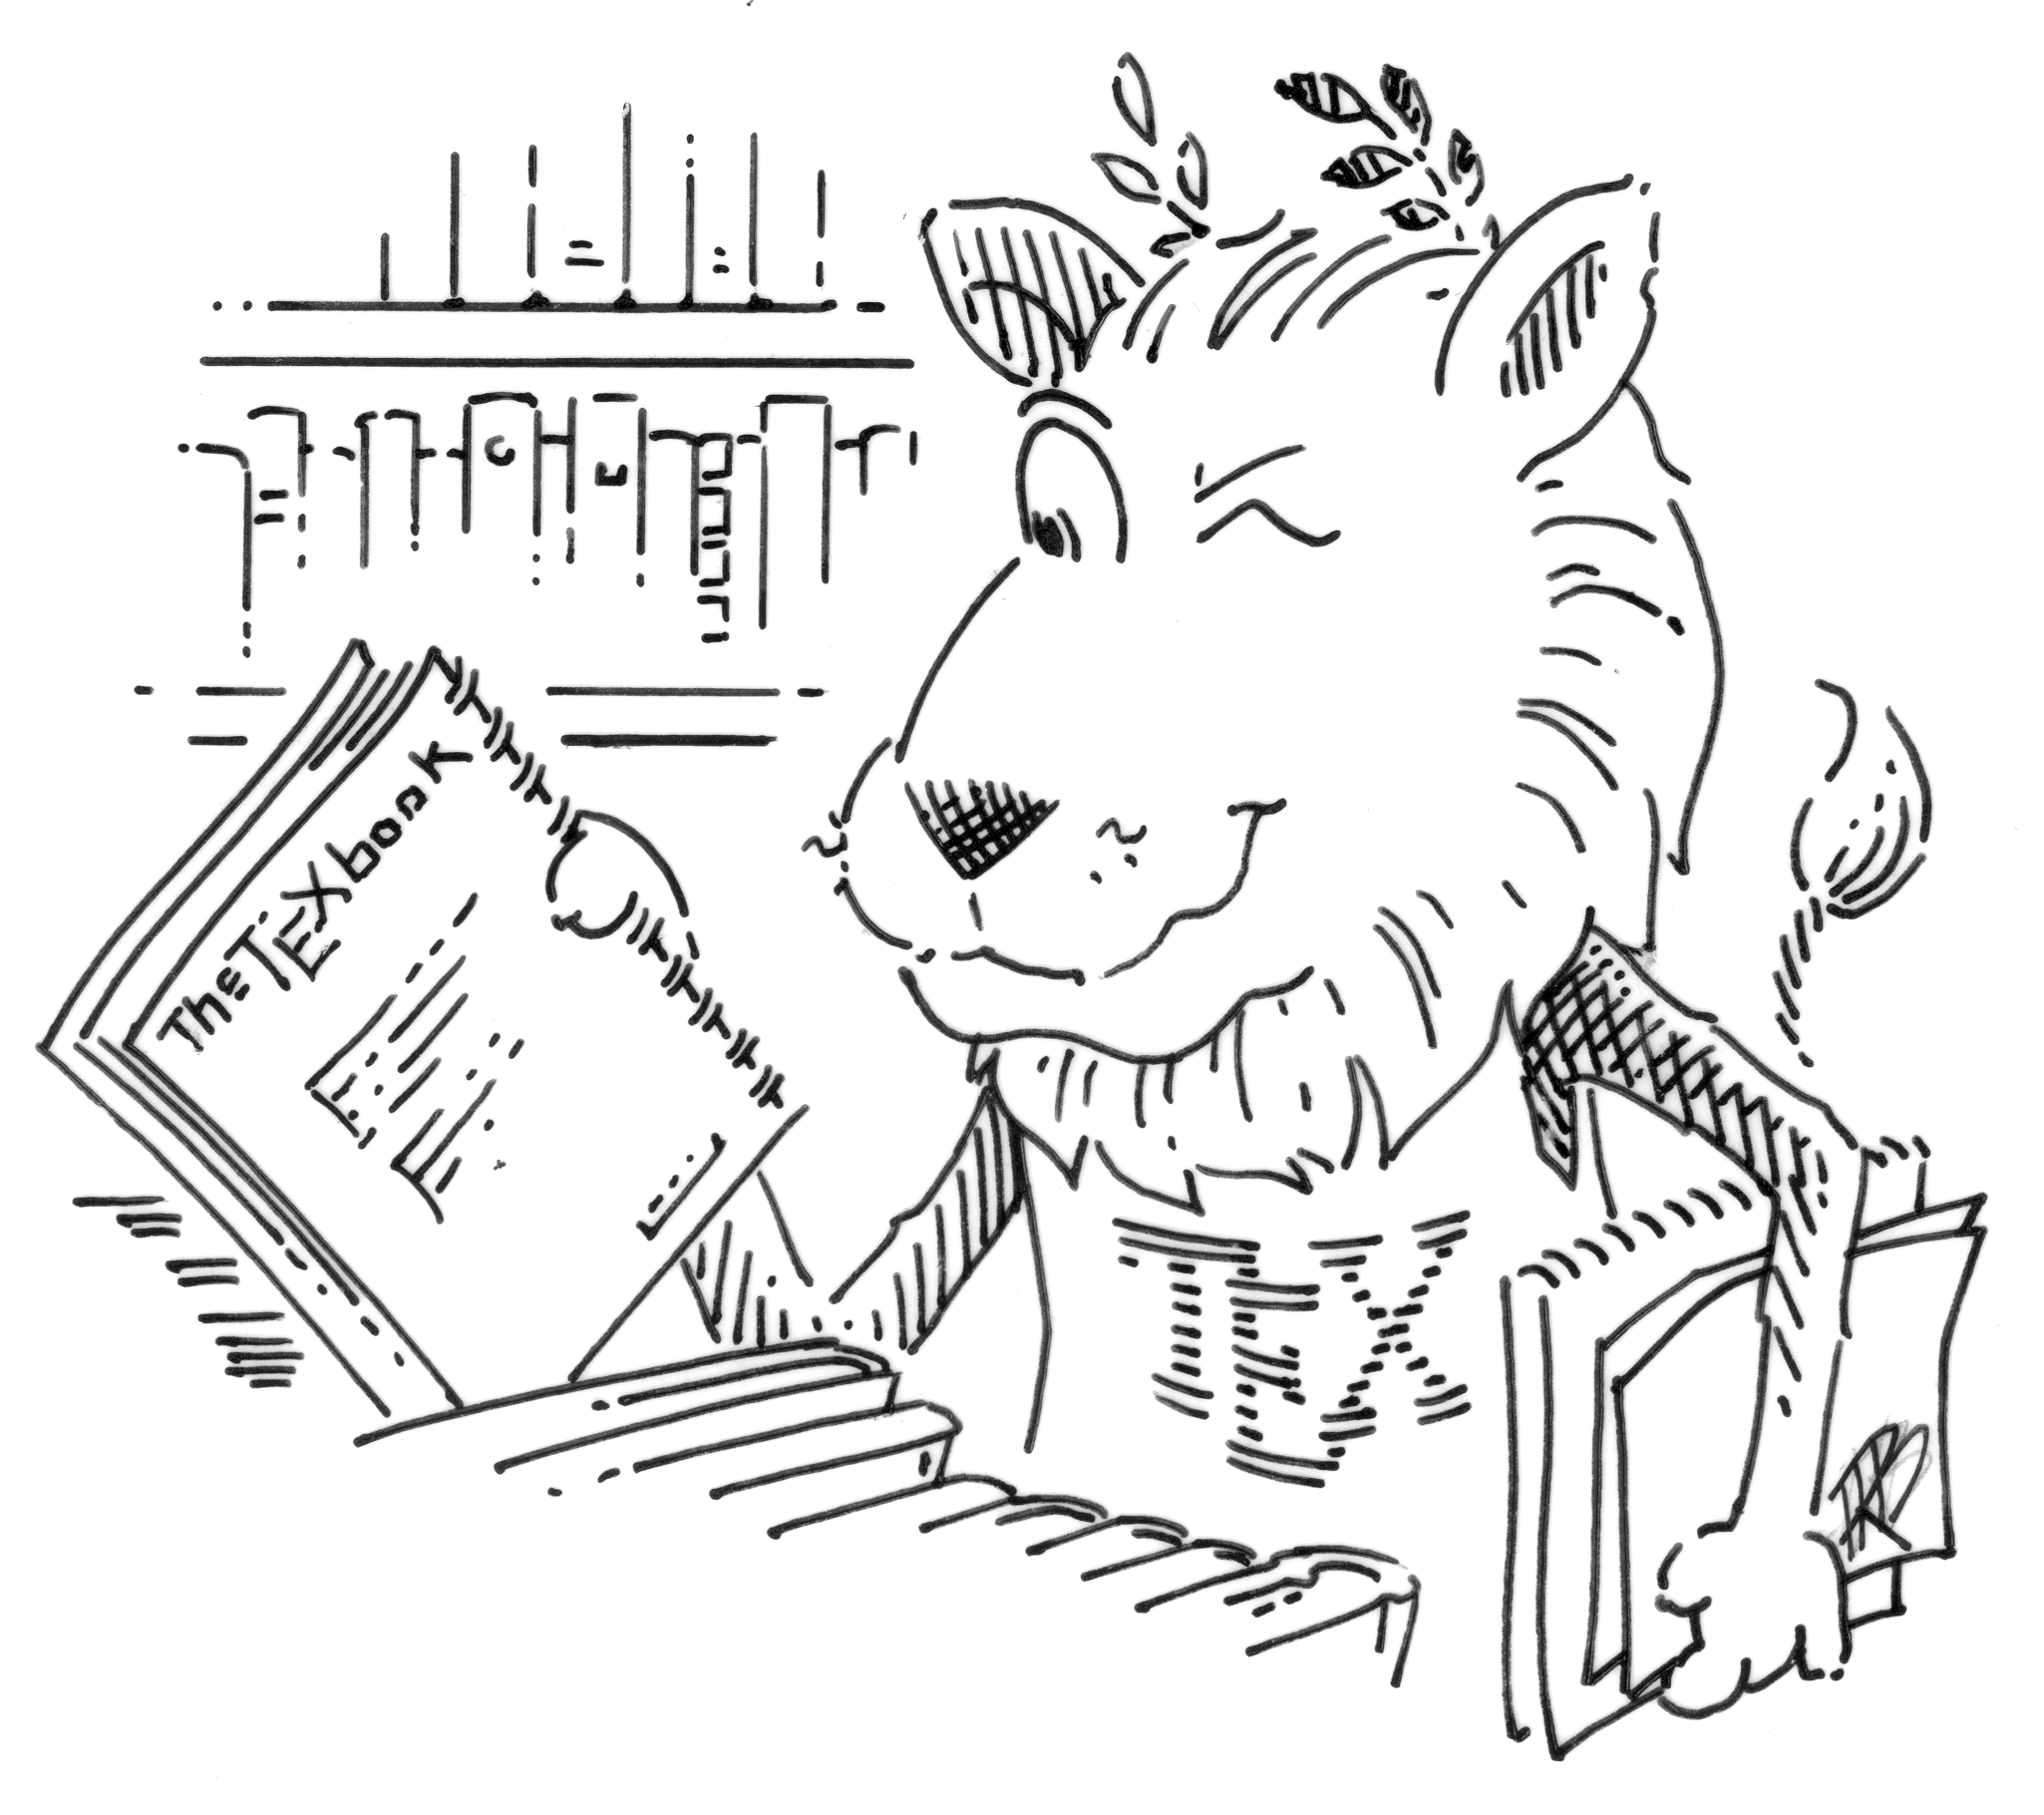
\includegraphics[scale=.040]{./img/tex-lion.png}
\end{multicols}

Outras opções, tais como imagens lado a lado, aumentar ou diminuir o tamanho, inserir imagem dentro de caixas de texto, etc, são indicadas no pacote.

%=======================================================
\chapter{Ambientes \LaTeX\ personalizados}

\subsection{citel}

\textsc{O que faz?}: Formata citações longas (com mais de três linhas) de acordo com a ABNT NBR 10520\footnote{A norma foi atualizada em 2023, informando que o recuo de citações longas não precisa ser \textsc{exatamente} 4cm da margem esquerda. No entanto, preferi manter a orientação anterior da norma que definia o recuo com essas medidas.}. Tem-se um recuo de 4cm da margem, tamanho da fonte 10pt e espaçamento simples entre linhas.

\begin{codex}{Código para citações longas}
	\begin{citel}
		Lorem ipsum dolor sit amet, consectetur adipiscing elit. Etiam at sapien erat. Donec nunc sem, sollicitudin id accumsan vitae, pharetra at eros. Etiam tellus erat, tempus feugiat cursus quis, vestibulum sit amet lacus. Praesent sed erat non erat accumsan aliquam. Duis volutpat tellus in erat venenatis vulputate. Aliquam at mauris vitae risus congue maximus sollicitudin nec velit. Duis rhoncus, urna in scelerisque mollis, libero augue viverra arcu, vel varius risus mi id felis. Mauris quis massa ac est finibus sodales at sed tortor. Aenean vel est nec purus finibus imperdiet.
	\end{citel}
\end{codex}

\textsc{Resultado:}

\begin{citel}
	Lorem ipsum dolor sit amet, consectetur adipiscing elit. Etiam at sapien erat. Donec nunc sem, sollicitudin id accumsan vitae, pharetra at eros. Etiam tellus erat, tempus feugiat cursus quis, vestibulum sit amet lacus. Praesent sed erat non erat accumsan aliquam. Duis volutpat tellus in erat venenatis vulputate. Aliquam at mauris vitae risus congue maximus sollicitudin nec velit. Duis rhoncus, urna in scelerisque mollis, libero augue viverra arcu, vel varius risus mi id felis. Mauris quis massa ac est finibus sodales at sed tortor. Aenean vel est nec purus finibus imperdiet.
\end{citel}

\subsection{codex}{Inserção de códigos de programação}

Depende do pacote \verb|tcolorbox|, que já vem ativado nesse modelo; porém, trata-se de um ambiente personalizado.

\textsc{O que faz?}: Permite a inserção de códigos de programação para demonstração.

Para este modelo de documento, criei um ambiente chamado \verb|codex| (CODigo de EXemplo). Esse ambiente é utilizado para todos os exemplos em que se demonstra o código \LaTeX. Suas características são:

\begin{enumerate}
	\item caixa de texto com moldura do título na cor cinza com letras brancas
	\item texto inicial do título: \textbf{Exemplo} + \textbf{numeração automática do exemplo conforme o capítulo ou seção onde se inseriu o ambiente}
	\item fundo da caixa de texto na cor cinza
	\item numeração de linhas automáticas para análise/estudo/demonstração do código
	\item ambiente verbatim na caixa de texto
\end{enumerate} 

Deve ser iniciado como abaixo:

\begin{verbatim}
	\begin{codex}{Digite aqui a identificação do exemplo. Obrigatório}
		insira aqui o que desejar
	\end{codex}
\end{verbatim}

\textsc{Resultado:}

\begin{codex}{Digite aqui a identificação do exemplo. Obrigatório}
	insira aqui o que desejar
\end{codex}

A seguir, um exemplo de código em Java\footnote{Retirado de \url{https://java.hotexamples.com/pt/examples/-/Average/-/java-average-class-examples.html}.}.

\begin{codex}{Exemplo de código em Java}
	/**
	* @param args
	* @throws FileNotFoundException
	*/
	public static void main(String[] args) throws FileNotFoundException {
		// TODO Auto-generated method stub
		System.out.println("Swim Meet Planner");
		
		// scanner to read file
		Scanner fileReader = new Scanner(new File("src/Finalprojectinput"));
		
		// create results Map
		HashMap<String, ArrayList<Integer>> results = new HashMap<String, ArrayList<Integer>>();
		
		// adding names and times to results Map
		while (fileReader.hasNext()) {
			String name = fileReader.next();
			int time = fileReader.nextInt();
			// does swimmer exist in map?
			if (results.containsKey(name)) {
				results.get(name).add(time);
				
			} else {
				ArrayList<Integer> times = new ArrayList<Integer>();
				times.add(time);
				results.put(name, times);
			}
		}
		fileReader.close();
		Average a = new Average();
		a.average(results);
	}
\end{codex}
\ \\

Caso não fosse utilizado o ambiente \verb|codex| e o código fosse digitado diretamente no editor, seu resultado seria \underline{impossível} em \LaTeX\ já que as chaves compõem a sintaxe do \LaTeX.

\fbox{Importante I:}

Caso você opte por considerar os exemplos de códigos como figuras, será necessário incluir o ambiente \verb|codex| dentro do ambiente \verb|figure| e adicionar, após \verb|\end{codex}| as seguintes linhas:

\begin{itemize}
	\item \verb|\caption|\{Nome do exemplo dado no título.\}
	\item \verb|\label{id:1}| - identificação da imagem para referência cruzada
\end{itemize}

Veja a seguir:

\begin{verbatim}
	\begin{figure}[h!]
	\begin{codex}{Ambiente codex em ambiente figure}
	arc=0mm,
	listing only,
	colback=black!5!white,
	colframe=black!85!white,
	fonttitle=\bfseries,
	title=Exemplo
	\end{codex}
	\caption{Ambiente codex em ambiente figure}
	\label{cod:1} % aqui é a id, seguida de : e a numeração
	\end{figure}
\end{verbatim}

\textsc{Resultado:}

\begin{figure}[h!]
\begin{codex}{Ambiente \{codex\} em ambiente \{figure\}}
arc=0mm,
listing only,
colback=black!5!white,
colframe=black!85!white,
fonttitle=\bfseries,
title=Exemplo
\end{codex}
\caption{Ambiente \{codex\} em ambiente \{figure\}}
\label{cod:1}
\end{figure}

Observe que a legenda já é inserida automaticamente e, também, esse exemplo já aparece na lista de figuras, no início do documento.

Caso se deseje referenciar essa figura ao longo do documento como referência cruzada, basta digitar \verb|\ref{cod:1}|, como aqui: \textit{O exemplo da figura \ref{cod:1} é do ambiente \{codex\} dentro do ambiente \{figure\}}.

\fbox{Importante II:}

Sempre alinhe o código na margem esquerda pois, caso o alinhamento fique com muitas tabulações, o código parecerá desorganizado (como o do Java acima).

\subsection{Caixas de Texto}

Além do pacote \verb|tcolorbox| e doo ambiente \verb|codex|, explicado anteriormente, há diversos \textbf{ambientes} possíveis nesse modelo para criar caixas de texto. São eles:

\subsubsection{observ}

\textsc{O que faz?} Produz uma caixa de texto com o título \qq{\textbf{Observação}} no topo para inserir... \textit{observações} que se julguem importantes. A fonte utilizada para o texto dentro da caixa é a mesma do documento.

\begin{codex}{Código para caixa para observações}
	\begin{observ}
	Aqui o texto muito importante para observações.
	\end{observ}
\end{codex}

\textsc{Resultado:}
\begin{observ}
	Aqui o texto muito importante para observações.
\end{observ}

\fbox{Observação:} 

Todos os ambientes a seguir produzem caixas de texto. Em alguns trabalhos acadêmicos o \textit{corpus} precisa ser exibido com diferentes formatações e, por isso, muitas devem ser diferenciados para facilitar a leitura. 

\subsubsection{mverde e mvermelha}

\textsc{O que fazem?} Produzem caixas de texto \textsc{com título} nas cores verde e vermelha, respectivamente:

\begin{codex}{Código para o ambiente mverde}
	\begin{mverde}{Título da caixa mverde}
	Note que a indicação do título é obrigatória.
	\end{mverde}
\end{codex}

\textsc{Resultado:}
\begin{mverde}{Título da caixa mverde}
	Note que a indicação do título é obrigatória.
\end{mverde}
\ \\

\begin{codex}{Código para o ambiente mvermelha}
	\begin{mvermelha}{Título da caixa mvermelha}
	Note que a indicação do título é obrigatória.
	\end{mvermelha}
\end{codex}

\textsc{Resultado:}
\begin{mvermelha}{Título da caixa mvermelha}
	Note que a indicação do título é obrigatória.
\end{mvermelha}
\ \\

\noindent\fbox{Não esquecer:} 

Para as caixas/os ambientes \verb|mverde| e \verb|mvermelha| o texto do título é obrigatório.

\subsubsection{bxpreta, bxlaranja, bxcinza, bxazul e bxvermelha}

As caixas seguintes não requerem título.

\begin{codex}{Ambiente bxpreta}
	\begin{bxpreta}
	Caixa de texto com moldura preta na lateral esquerda. 
	
	Mais algum texto para complementar.   
	\end{bxpreta} 
\end{codex}

\textsc{Resultado:}
\begin{bxpreta}
	Caixa de texto com \textbf{moldura preta} na lateral esquerda. 
	
	Mais algum texto para complementar.     
\end{bxpreta} 
\ \\

\begin{codex}{Ambiente bxlaranja}
	\begin{bxlaranja}
	Caixa de texto com \textbf{moldura laranja} na lateral esquerda.  
	
	Mais algum texto para complementar.  
	\end{bxlaranja}
\end{codex}

\textsc{Resultado:}
\begin{bxlaranja}
	Caixa de texto com \textbf{moldura laranja} na lateral esquerda.
	
	Mais algum texto para complementar.   
\end{bxlaranja}
\ \\

\begin{codex}{Ambiente bxcinza}
	\begin{bxcinza}
	Caixa de texto com \textbf{moldura cinza} na lateral esquerda. 
	
	Mais algum texto para complementar.  
	\end{bxcinza}
\end{codex}

\textsc{Resultado:}
\begin{bxcinza}
	Caixa de texto com \textbf{moldura cinza} na lateral esquerda. 
	
	Mais algum texto para complementar.  
\end{bxcinza}
\ \\

\begin{codex}{Ambiente bxazul}
	\begin{bxazul}
	Caixa de texto com \textbf{moldura azul} na lateral esquerda. 
	
	Mais algum texto para complementar.  
	\end{bxazul}
\end{codex}

 \textsc{Resultado:}
\begin{bxazul}
	Caixa de texto com \textbf{moldura azul} na lateral esquerda. 
	
	Mais algum texto para complementar.  
\end{bxazul}
\ \\

\begin{codex}{Ambiente bxvermelha}
	\begin{bxvermelha}
	Caixa de texto com \textbf{moldura vermelha} na lateral esquerda. 
		
	Mais algum texto para complementar.  
	\end{bxvermelha}
\end{codex}

\textsc{Resultado:}
\begin{bxvermelha}
	Caixa de texto com \textbf{moldura vermelha} na lateral esquerda. 
	
	Mais algum texto para complementar.  
\end{bxvermelha}


\subsubsection{alertmessage}

\textsc{Qual o pacote?}: alertmessage (Acesso: \url{https://www.ctan.org/pkg/alertmessage})

Trata-se esse pacote de um \textit{comando} e não de um ambiente.

\textsc{O que faz?}: Produz caixas de texto com as seguintes especificações.

\begin{itemize}
\item caixa azul, com ícone "i".
\item caixa verde com ícone de "confere".
\item caixa vermelha com ícone de "x" ou "erro".
\item caixa laranja com ícone de"!" ou exclamação.
\end{itemize}


\begin{codex}{Todos os comandos para alertmessage}
	A. \alertinfo{caixa azul, com ícone "i"}
	B. \alertsuccess{caixa verde com ícone de "confere"}
	C. \alerterror{caixa vermelha com ícone de "x" ou "erro"}
	D. \alertwarning{caixa laranja com ícone de"!" ou exclamação}
\end{codex}

\textsc{Resultado:}

A. \alertinfo{caixa azul, com ícone "i".}

B. \alertsuccess{caixa verde com ícone de "confere".}

C. \alerterror{caixa vermelha com ícone de "x" ou "erro".}

D. \alertwarning{caixa laranja com ícone de"!" ou exclamação.}


%=======================================================
\chapter{Referências e Citações}

Citações e referências no \LaTeX\ podem ser trabalhosas principalmente em razão da \qq{loucura} que são as normas ABNT para trabalhos acadêmicos. Sem adentrar muito na questão, menciono apenas que os pacotes para citação e referência aqui utilizados já estão em vias de se tornarem \qq{obsoletos} por causa da recente modificação (em 2023) das normas para citação (ABNT NBR 10520). Além disso, as referências (ABNT NBR 6023), cuja atualização em 2018 e correção em 2020, também sofreram modificações segundo a norma. Enfim, vamos ao que interessa.

Referências em \LaTeX\ são feitas em um arquivo à parte, cuja a extensão é | .bib |. Nesse projeto, o arquivo das referências chama-se \verb|referencias.bib|.

Para cada tipo de referência - livro, artigo, capítulo de livro, sites, revistas, etc - existe uma entrada específica, isto é, um formato específico de registrar a referência.

O exemplo a seguir é de um livro com apenas um autor. O código à esquerda é vazio e o segundo, á direita, a referência já preenchida\footnote{Ignorem a não obediência à margem. O ambiente \textit{verbatim} não a respeita.}. Em seguida, explico cada uma das linhas.

\begin{multicols}{2}
\begin{verbatim}
	@book{, 
		author     = {},
		title      = {},
		edition    = {},
		address    = {},
		publisher  = {},
		year       = {},
		translator = {},
	}
\end{verbatim}

\begin{verbatim}
@book{todorov2014, 
author     = {Tzvetan Todorov },
title      = {Simbolismo e interpretação},
edition    = {1},
address    = {São Paulo},
publisher  = {Editora UNESP},
year       = {2014},
translator = {Nícia Adan Bonatti},
}
\end{verbatim}
\end{multicols}


{\textbf{@book{todorov2014,}} - Inicia-se a entrada com @ seguida do tipo (nesse caso, \textit{book}). Em seguida, abre-se a chave e inclui-se a identificação (ou chave de entrada), separando-a dos demais campos com uma vírgula ( , ). Essa chave pode ser o que quiser, desde que sirva para identifica o trabalho.
	
{\textbf{author     = \{\},}} - Indica-se o nome do autor. O pacote utilizado (\verb|abntex2cite|) requer atenção às palavras acentuadas. Veja a documentação do pacote para uso de palavras acentuadas na construção das referências.

{\textbf{title      = \{\},}} - Indica-se o título do trabalho. Idem em relação ao uso de acentos.

{\textbf{edition    = \{\},}} - Indica-se o número da edição. Se não houver, deixa-se em branco.

{\textbf{address    = \{\},}} - Indica-se o local da publicação. Essa informação encontra-se na ficha catalográfica do livro.

{\textbf{publisher  = \{\},}} - Indica-se a editora resposnável pela publicação do livro.

{\textbf{year       = \{\},}} - Indica-se o ano de publicação.

{\textbf{translator = \{\},}} - - Indica-se quem traduziu a obra. Se não houver, deixa-se em branco.

É preciso obedecer às chaves e vírgulas, caso contrário, no momento da compilação, haverá erro.

Para a utilização correta do pacote \verb|abntex2cite| nesse projeto, é essencial a leitura dos seguintes materiais disponíveis em \url{https://www.ctan.org/pkg/abntex2}, em especial:

\begin{itemize}
    \item \url{https://linorg.usp.br/CTAN/macros/latex/contrib/abntex2/doc/abntex2cite.pdf}
    \item \url{https://linorg.usp.br/CTAN/macros/latex/contrib/abntex2/doc/abntex2cite-alf.pdf}
\end{itemize}

Ambos os pacotes contém exemplos de uso e, também, a acentuação necessária para cada entrada bibliográfica que deve ser inserida no arquivo \verb|referencias.bib|.

Há, também, um gerador \textit{online} de referências em \LaTeX. O endereço é \url{https://truben.no/latex/bibtex/}. No entanto, advirto que existe a possibilidade de erro porque os campos do pacote \verb|abntex2cite|, aqui utilizado, não são os mesmos gerados por esse \textit{site}. Nada impede o teste!!!

Após construída a lista de referências (ou o banco de dados de referências), é possível citar as obras no texto. Citar \qq{manualmente} a uma referência e depois incluí-la no arquivo .bib fará p \LaTeX\ ignorar tal referência. isso porque somente se referencia o que se cita no texto e, como o \LaTeX\ faz por você esse processo, ele o faz também com as citações.

Vejamos um exemplo. No arquivo \verb|referencias.bib| existe a seguinte entrada de exemplo:

\begin{verbatim}
	@article{Smurf1980,
		author  = {Papai Smurf},
		title   = {Como preparar trufas azuis},
		journal = {The Smurfs Newsletters},
		ISSN    = {123-456-789},
		volume  = {1},
		number  = {1},
		month   = {Jan.},
		year    = {1980},
		pages   = {1-10},
		doi     = {http://doi.com.com},
		url     = {http://www.thesmurfs.com.com},
		urlaccessdate = {10 jun. 1981},
	}
\end{verbatim}

Se eu optar por citar de modo manual, por exemplo, assim: 
\ \\

\textit{De acordo com Smurf (1980), as trufas são deliciosas e por isso Gargamel as quer.}
\ \\
Porém, se eu citar utilizando o comando próprio de citações (\verb|\cite|), após a compilação, a referência será incluída na seção \textbf{Referências} conforme a ABNT NBR 6023. Por exemplo

\textit{De acordo com \cite{Smurf1980}, as trufas são deliciosas e por isso Gargamel as quer.}

Observe que agora a citação aparece em cor azul, está \textit{hiperlinkada} apontando diretamente para a referência na seção... \textbf{Referências}!!!

Os comandos para citar são: 
\begin{itemize}
	\item \verb|\cite{chave_de_entrada}| e 
	\item \verb|\citeonline{chave_de_entrada}|. 
\end{itemize}

O primeiro é utilizado para citações diretas enquanto o segundo, para citações indiretas.

Nos dois casos é possível indicar o número da página desta forma:

\begin{codex}{Códigos para citações incluindo a página}
\cite[p. 35]{Flintstones1900}

\citeonline[págs. 25-50]{Thor2017}
\end{codex}

\textsc{Resultado:}

Assim, vemos que não é \qq{sempre que se come uma carne de tiranossauro rex com temperos indianos} \cite[p. 35]{Flintstones1900}.

Foi, de fato, algo inesperado. Como nos lembrou \citeonline[págs. 25-50]{Thor2017}, o martelo estava sem controle absoluto e eu não se pode fazer nada.
%===============================
%INÍCIO DOS ELEMENTOS PÓS TEXTUAIS (REFERÊNCIAS, ANEXOS, APÊNDICES)

\backmatter{
%Início das Referências
\renewcommand{\bibname}{Referências}
\bibintoc
\bibliographystyle{abntex2-alf}
\bibliography{referencias.bib}
%Fim das Referências

%Se o trabalho não tiver apêndices ou anexos
%excluir ou comentar a linha abaixo.
%ANEXOS
\thispagestyle{empty}
\part*{Anexos} % Se quiser uma página indicativa de ANEXOS antes dos anexos.
\addcontentsline{toc}{part}{Anexos}
%Conforme a norma, os anexos devem se organizar em ordem alfabética: A, B, C, D...
\chapter*{Anexo A -- Um anexo}
\addcontentsline{toc}{chapter}{Anexo A -- Um anexo}


%APÊNDICES
\thispagestyle{empty}
\part*{Apêndices} % se quiser uma página indicativa de APÊNDICES antes dos apêndices
\addcontentsline{toc}{part}{Apêndices}
%Conforme a norma, os apêndices devem se organizar em ordem alfabética: A, B, C, D...
\chapter*{Apêndice A -- lettrine}
\addcontentsline{toc}{chapter}{Apêndice A -- lettrine}

\noindent\textsc{O que faz?}

Desenha uma caixa de texto ao redor da primeira letra da primeira palavra do parágrafo. É um recurso de estilo, apenas.

\lettrine[findent=2pt]{\fbox{\textbf{V}}}{eja essa frase de abertura...} \lipsum[1]

\chapter*{Apêndice B -- verbatim}
\addcontentsline{toc}{chapter}{Apêndice A -- verbatim}

\noindent\textsc{O que faz?}

Digita qualquer coisa fora da formatação do texto, utilizando fonte monoespaçada e conforme os espaçamentos desejados. Útil para pequenos trechos de código.

\begin{codex}{Códigos verbatim}
\verb|comando 1|
    \verb*|comando 2]
        \begin{verbatim}
            qualquer outro texto
        \end{verbatim}
\begin{mverbt}
ambiente personalizado
\item um item de lista
\end{mverbt}
\end{codex}
\begin{multicols}{2}
\setlength{\columnseprule}{0.2pt}
O comando da linha 1, gera o seguinte: \verb|comando 1|.

O comando da linha 2, gera o seguinte: \verb*|comando 2].

Os comandos das linhas 3, 4 e 5 geram o seguinte:
\begin{verbatim}
   qualquer outro texto
\end{verbatim}

Os comandos das linhas 6, 7, 8 e 9 geram o seguinte:
        \begin{mverbt}
        ambiente personalizado
        \item um item de lista
        \end{mverbt}
\end{multicols}
\textbf{Observação:} Notar o alinhamento dos dois últimos ambientes. A tabulação na digitação -- \textit{em verbatim} -- importa para o \LaTeX.


\chapter*{Apêndice C -- pdfpages}
\addcontentsline{toc}{chapter}{Apêndice C -- pdfpages}

\noindent\textsc{O que faz?}

Insere uma ou várias páginas .pdf no arquivo gerado pelo \LaTeX. A numeração é feita de modo automático.

Veja a numeração desta página, note a figura inserida do Tex the Lion e a numeração do \textbf{Apêndice D}. 

Observar o código:
\ \\
\begin{codex}{Inserção de página pdf - Tex the Lion}
    
\includepdf[noautoscale=false]{img/tex-lion.pdf}
\end{codex}


\includepdf[noautoscale=false]{img/tex-lion.pdf}

\chapter*{Apêndice D -- multicol}
\addcontentsline{toc}{chapter}{Apêndice D -- multicol}

\noindent\textsc{O que faz?}

Divide o texto em -- \textit{no máximo} -- 10 colunas. No \textbf{Apêndice C}, tem-se alguns exemplos com o ambiente verbatim.

Observar:

\begin{codex}{Multicolunas com valor 3 e Lorem Ipsum}
    \begin{multicols}{3}
        \lipsum[2]
    \end{multicols}
\end{codex}

\begin{multicols}{3}
        \lipsum[2]
    \end{multicols}

\begin{codex}{Multicolunas com valor 5 e Lorem Ipsum}
    \begin{multicols}{5}
        \lipsum[2]
    \end{multicols}
\end{codex}

\begin{multicols}{5}
        \lipsum[2]
   \end{multicols}

Também é possível incluir uma linha separadora entre as colunas. Ver a seguir.

\begin{codex}{Multicolunas com valor 3 e Lorem Ipsum + Linha}
    \begin{multicols}{3}
    \setlength{\columnseprule}{0.2pt}
    \lipsum[2]
    \end{multicols}
\end{codex}

 \begin{multicols}{3}
    \setlength{\columnseprule}{0.2pt}
    \lipsum[2]
 \end{multicols}

\chapter*{Apêndice E -- smartdiagram}
\addcontentsline{toc}{chapter}{Apêndice E -- smartdiagram}

\noindent\textsc{O que faz?}

Cria diagramas coloridos, em escala de cinza, branco e preto, em formatos diversos a partir de uma lista de itens simples.

\begin{codex}{circular diagram}
\begin{center}
\smartdiagram[circular diagram]{\LaTeX,Digitar,Compilar,Produzir PDF}
\end{center}	
\end{codex}

\begin{center}
	\smartdiagram[circular diagram]{\LaTeX,Digitar,Compilar,Produzir PDF}
\end{center}

\chapter*{Apêndice F -- textcmds}
\addcontentsline{toc}{chapter}{Apêndice F -- textcmds}

\noindent\textsc{O que faz?}
Permite incluir aspas duplas e simples, e outros símbolos tipográficos, com menos esforço na digitação.

Por padrão, o \LaTeX\ produz aspas das seguintes formas:
\begin{enumerate}
	\item SHIFT + acento grave 2x + SHIFT + acento grave 2x + palavra ou expressão entre aspas + aspas simples 2x.
            \begin{itemize}
                \item 'um texto qualquer' entre aspas simples
            \end{itemize}
	\item SHIFT + sinal de acento grave + palavra ou expressão + aspas simples.
            \begin{itemize}
                \item "um texto qualquer" entre aspas duplas
            \end{itemize}
\end{enumerate}

No primeiro exemplo, o 1º sinal das aspas simples não está correto, pois deveria estar voltado para direita.

No segundo exemplo, quando compilado fora do Overleaf, não acrescenta o espaço entre as últimas aspas duplas e a próxima palavra.

Para resolver isso e utilizar \textit{on-line} e \textit{offline} ambas as aspas, use os comandos:

\begin{codex}{Aspas com o pacote textcmds}
Estas são \qq{aspas duplas}.
Estas são \q{aspas simples}.
Estas são \qq{aspas duplas com \q{aspas simples} ao mesmo tempo}
\end{codex}
 Produzirão, respectivamente: Estas são \qq{aspas duplas}; Estas são \q{aspas simples} e Estas são \qq{aspas duplas com \q{aspas simples} ao mesmo tempo}.


\chapter*{Apêndice G -- xurl}
\addcontentsline{toc}{chapter}{Apêndice G -- xurl}

\noindent\textsc{O que faz?}
Permite a quebra de \textit{urls} mesmo quando existem caracteres como \&, \_, \#.

Observe que  caixa de texto, por ser -- também -- um ambiente verbatim, não \qq{quebrará} a url, porém quando digitado em ambiente não verbatim, o endereço é ajustado automaticamente conforme as margens.

\begin{codex}{Exemplo de url longa}
  \url{https://tex.stackexchange.com/questions/341205/what-is-the-difference-between-tabular-tabular-and-tabularx-environments}
\end{codex}
\ \\
Endereço URL ajustado a seguir:

\url{https://tex.stackexchange.com/questions/341205/what-is-the-difference-between-tabular-tabular-and-tabularx-environments}

\chapter*{Apêndice H -- tabularx e booktabs}
\addcontentsline{toc}{chapter}{Apêndice H -- tabularx e booktabs}

\noindent\textsc{O que faz?}

Ambos permitem maior controle de personalização nas tabelas. Reproduzo somente uma simples tabela para fins de estudo do código.

\begin{codex}{Tabela com legenda e referência cruzada}
\begin{table}[h!]
    \begin{center}
	\begin{tabularx}{0.8\textwidth} { 
	| >{\centering\arraybackslash}X 
	| >{\centering\arraybackslash}X 
	| >{\centering\arraybackslash}X | }
	\hline
	item 1 & item 2 & item 3 \\
	\hline
	item 4  & item 5  & item 6  \\
	\hline
	\end{tabularx}
	\caption{Tabela de teste. Abaixo, a ref. cruzada.}
	\label{table:1}
	\end{center}
\end{table}
\end{codex}

\begin{table}[h!]
    \begin{center}
	\begin{tabularx}{0.8\textwidth} { 
	| >{\centering\arraybackslash}X 
	| >{\centering\arraybackslash}X 
	| >{\centering\arraybackslash}X | }
	\hline
	item 1 & item 2 & item 3 \\
	\hline
	item 4  & item 5  & item 6  \\
	\hline
	\end{tabularx}
	\caption{Tabela de teste. Abaixo, a ref. cruzada.}
	\label{table:1}
	\end{center}
\end{table}

E a ref. cruzada se faz com \verb|\ref{table:1}|, e fica \textit{hiperlinkado} para a Tabela \ref{table:1}.

\chapter*{Apêndice I -- graphix}
\addcontentsline{toc}{chapter}{Apêndice I -- graphix}

\noindent\textsc{O que faz?}

Insere imagens nos formatos JPG, PNG, PDF ou EPS. Demonstro somente como incluir uma imagem centralizada na página.

\begin{codex}{Código para inserção de imagens}
\begin{figure}[h!]
	\begin{center}
		
\includegraphics[scale=.30]{./img/github.png}
		\caption{Imagem GitHub}
		\label{fig:github}
	\end{center}
\end{figure}
\end{codex}

\begin{figure}[h!]
	\begin{center}
		
\includegraphics[scale=.30]{./img/github.png}
		\caption{Imagem GitHub}
		\label{fig:github}
	\end{center}
\end{figure}

Outras opções, tais como imagens lado a lado, aumento do tamanho, dentro de caixas de texto, etc, são indicadas no pacote.


\chapter*{Apêndice I -- Inserção de códigos de programação}
\addcontentsline{toc}{chapter}{Apêndice I -- Inserção de códigos de programação}

\noindent\textsc{O que faz?}

Insere códigos de programação com opções diferentes conforme o pacote utilizado. 

Neste modelo criei um ambiente chamado \verb|codex| que é o utilizado para todos os exemplos. Sua características são:

\begin{enumerate}
    \item caixa de texto com moldura do título preta com letras brancas
    \item texto inicial do título: \textbf{Exemplo} + \textbf{numeração da seção onde se inseriu o ambiente}
    \item fundo da caixa de texto na cor cinza
    \item numeração de linhas automáticas para análise/estudo/demonstração do código
    \item ambiente verbatim na caixa de texto
\end{enumerate} 

O ambiente \verb|codex| será o primeiro a ser exemplificado.

\textsc{Ambiente codex:} o que está dentro da primeira caixa (3.11) produzirá a segunda caixa (3.12)\footnote{Observe o espaço \textsc{intencional} entre as palavras.}.

\begin{codex}{Exemplo do exemplo}
\begin{codex}{Título de exemplo do ambiente (obrigatório)}
    aqui irá o código
        de      exemplo
    com     objetivo    de      exemplificar
\end{codex}
\end{codex}

\begin{codex}{Título de exemplo do ambiente (obrigatório)}
    aqui irá o código
        de      exemplo
    com     objetivo    de      exemplificar
\end{codex}

\newpage
\textsc{Pacote codebox}

\begin{codex}{Exemplo de uso: CODEBOX}
    \begin{codebox}{CodeBox Title}
    #include <stdio.h>
    #include <stdlib.h>
    int main(void)
    {
    printf("Hello World!\n");
    return 0;
    }
    \end{codebox}
\end{codex}

    \begin{codebox}{CodeBox Title}
    #include <stdio.h>
    #include <stdlib.h>
    int main(void)
    {
    printf("Hello World!\n");
    return 0;
    }
    \end{codebox}

\begin{codex}{Exemplo de uso: CODEVIEWER}
\begin{codeview}{CodeViewer Title}
#include <stdio.h>
#include <stdlib.h>
int main(void)
{
printf("Hello World!\n");
return 0;
}
\end{codeview}

\end{codex}
\begin{codeview}{CodeViewer Title}
#include <stdio.h>
#include <stdlib.h>
int main(void)
{
printf("Hello World!\n");
return 0;
}
\end{codeview}

\newpage
\textsc{Pacote: shdoc} (para usuários Linux)

Há diversas maneiras de utilizar o \verb|shdoc|. Utilizei um exemplo apresentado na pág. 7 do \href{https://linorg.usp.br/CTAN/macros/latex/contrib/shdoc/shdoc.pdf}{manual}.

\begin{enumerate}
    \item digitei no shell: \verb|cat --help > cat-out.save|
    \item fiz upload da saída para esse projeto
    \begin{itemize}
        \item arq. cat-out.save
    \end{itemize}
    \item executei o comando \verb|\shread{cat --help}{cat-out.save}|
    \item (não\footnote{Antes de demonstrar o pacote pygmentex (caixa acima), o Overleaf compilou o comando sem problemas e exibiu uma imagem da saída do \textit{shell}. Compatibilidade dos pacotes? Questões do Overleaf?}) obtive a imagem abaixo
\end{enumerate}

O comando \verb|\shread{cat --help}{cat-out.save}| apresentou um erro no Overleaf. Sugiro testar \textit{offline}.

\textsc{Pacote: pygmentex}

\begin{codex}{Pygmentex - pág. 2 do manual}
    \begin{pygmented}[lang=c]
    #include <stdio.h>
    int main(void)
    {
    int a, b, c;
    printf("Enter two numbers to add: ");
    scanf("%d%d", &a, &b);
    c = a + b;
    printf("Sum of entered numbers = %d\n", c);
    return 0;
    }
    \end{pygmented}
\end{codex}

O ambiente acima apresentou um erro no Overleaf. Sugiro testar \textit{offline}


\chapter*{Apêndice J -- Ambientes \LaTeX\ personalizados}
\addcontentsline{toc}{chapter}{Apêndice J -- Ambientes \LaTeX\ personalizados}

\textsc{Ambiente \textbf{citel}}
\noindent\textsc{O que faz?}

Formata as citações longas, isto é, com mais de três linhas (de acordo com a ABNT) de modo adequado no \LaTeX. Recuo de 4cm à esquerda da margem, espaçamento simples e fonte de 10pt.

\begin{codex}{Citação com blá blá}
    \begin{citel}
    blá blá blá blá blá blá blá blá blá blá blá blá blá blá blá blá blá blá blá blá blá blá blá blá blá blá blá blá blá blá blá blá blá blá blá blá blá blá blá blá blá blá blá blá blá blá blá blá blá blá blá blá blá blá blá blá blá blá blá blá blá blá blá blá blá blá blá blá blá blá blá blá blá blá blá blá blá blá blá blá blá blá blá blá blá blá blá blá blá blá blá blá blá blá blá blá blá blá blá blá blá blá blá blá blá blá blá blá blá blá blá blá blá blá blá blá blá blá blá blá blá blá blá blá blá blá blá blá blá blá (FONTE, p. 1, 2020)
\end{citel}
\end{codex}

\begin{citel}
    blá blá blá blá blá blá blá blá blá blá blá blá blá blá blá blá blá blá blá blá blá blá blá blá blá blá blá blá blá blá blá blá blá blá blá blá blá blá blá blá blá blá blá blá blá blá blá blá blá blá blá blá blá blá blá blá blá blá blá blá blá blá blá blá blá blá blá blá blá blá blá blá blá blá blá blá blá blá blá blá blá blá blá blá blá blá blá blá blá blá blá blá blá blá blá blá blá blá blá blá blá blá blá blá blá blá blá blá blá blá blá blá blá blá blá blá blá blá blá blá blá blá blá blá blá blá blá blá blá blá (FONTE, p. 1, 2020)
\end{citel}

\newpage
\textsc{Ambiente \textbf{codex}}
\noindent\textsc{O que faz?}

Ver \textbf{Apêndice I} para explicações deste ambiente.

\textsc{Ambiente \textbf{observ}}
\noindent\textsc{O que faz?}

Produz uma caixa de texto com o título "\textbf{Observação}" no topo para inserir... \textit{observações} que se julguem importantes. A fonte utilizada para o texto dentro da caixa é a mesma do documento.

\begin{codex}{Caixa para observações}
    \begin{observ}
        Aqui o texto muito importante para observações.
    \end{observ}
\end{codex}
\ \\

\begin{observ}
        Aqui o texto muito importante para observações.
    \end{observ}


\chapter*{Apêndice K -- Caixas de texto}
\addcontentsline{toc}{chapter}{Apêndice K -- Caixas de texto}

\noindent\textsc{O que faz?}

Todos os ambientes a seguir produzem caixas de texto. Em alguns trabalhos acadêmicos o \textit{corpus} é exibido com diferentes formatações e, por isso, muitas vezes precisam ser diferenciados para facilitar a leitura. 

Os ambientes nesse modelo são\footnote{Os ambientes 1 e 2 já foram exemplificados. Ver Apêndices I e J.}:

\begin{enumerate}
    \item codex
    \item observ
    \item mverde
    \item mvermelha
    \item bxpreta
    \item bxlaranja
    \item bxcinza
    \item bxazul
    \item bxvermelha
    \item \textbf{alertmessage\footnote{Exceção aos listados acima. Trata-se de um comando, não de um ambiente.}}
\end{enumerate}

Seguindo a ordem numérica acima, seguem-se os exemplos.

\begin{codex}{Ambiente mverde}
\begin{mverde}{Título da caixa mverde}
    Note que a indicação do título é obrigatória.
\end{mverde}
\end{codex}

\begin{mverde}{Título da caixa mverde}
    Note que a indicação do título é obrigatória.
\end{mverde}

\begin{codex}{Ambiente mvermelha}
\begin{mvermelha}{Título da caixa mvermelha}
    Note que a indicação do título é obrigatória.
\end{mvermelha}
\end{codex}

\begin{mvermelha}{Título da caixa mvermelha}
    Note que a indicação do título é obrigatória.
\end{mvermelha}

\textsc{Atenção:} para as caixas/os ambientes \verb|mverde| e \verb|mvermelha| o texto do título é obrigatório.

As caixas seguintes não requerem título. Primeiro apresenta-se o código, em seguida o que é produzido/gerado para o pdf.

\begin{codex}{Ambiente bxpreta}
\begin{bxpreta}
Caixa de texto com moldura preta na lateral esquerda.    
\end{bxpreta} 
\end{codex}
.
\begin{bxpreta}
Caixa de texto com \textbf{moldura preta} na lateral esquerda.    
\end{bxpreta} 

\begin{codex}{Ambiente bxlaranja}
    \begin{bxlaranja}
        Caixa de texto com \textbf{moldura laranja} na lateral esquerda.  
    \end{bxlaranja}
 \end{codex}
.
\begin{bxlaranja}
        Caixa de texto com \textbf{moldura laranja} na lateral esquerda.  
\end{bxlaranja}


\begin{codex}{Ambiente bxcinza}
    \begin{bxcinza}
      Caixa de texto com \textbf{moldura cinza} na lateral esquerda. 
    \end{bxcinza}
\end{codex}
.
\begin{bxcinza}
      Caixa de texto com \textbf{moldura cinza} na lateral esquerda. 
\end{bxcinza}


\begin{codex}{Ambiente bxazul}
    \begin{bxazul}
      Caixa de texto com \textbf{moldura azul} na lateral esquerda. 
    \end{bxazul}
\end{codex}
.
\begin{bxazul}
      Caixa de texto com \textbf{moldura azul} na lateral esquerda. 
\end{bxazul}

\begin{codex}{Ambiente bxvermelha}
    \begin{bxvermelha}
      Caixa de texto com \textbf{moldura vermelha} na lateral esquerda. 
    \end{bxvermelha}
\end{codex}
.
\begin{bxvermelha}
   Caixa de texto com \textbf{moldura vermelha} na lateral esquerda. 
\end{bxvermelha}

Os últimos exemplos não são ambientes, mas comandos do pacote \verb|alertmessage| incluído nesse modelo de documento.

\begin{codex}{Todos os comandos para alertmessage}
    A. \alertinfo{caixa azul, com ícone "i"}
    B. \alertsuccess{caixa verde com ícone de "confere"}
    C. \alerterror{caixa vermelha com ícone de "x" ou "erro"}
    D. \alertwarning{caixa laranja com ícone de"!" ou exclamação}
\end{codex}

    A. \alertinfo{caixa azul, com ícone "i".}

    B. \alertsuccess{caixa verde com ícone de "confere".}
    
    C. \alerterror{caixa vermelha com ícone de "x" ou "erro".}
    
    D. \alertwarning{caixa laranja com íncone de"!" ou exclamação.}

%Comando para gerar folha de guarda (pág. em branco ao final)
\newpage
\thispagestyle{empty}
\mbox{}
\newpage
%FIM DOS ELEMENTOS TEXTUAIS (CAPS./SEÇÕES)
%Não apagar a chave a seguir.
}
%FIM DOS ELEMENTOS PÓS TEXTUAIS (REFERÊNCIAS, ANEXOS, APÊNDICES)
\end{document}
